In this chapter we will explore the mathematical structure of symmetry in the software synthesis process, mostly the work published in ~\cite{goens_iess15,goens_taco17,goens_scopes17,goens_mcsoc18,goens_tcad21}.
The material in this section makes use of concepts in group theory.
We assume the basic concepts as seen in any undergraduate course on group
theory, with the definitions of groups, actions and orbits.
A brief introduction, to the level required by this chapter, can be found in Appendix~\ref{appendix:groups}. 

\subsection{Architectures and Applications}
\label{sec:arch_app_symmetries}

Intuitively, when we say an object is very symmetric we usually mean it has parts that are similar or identic, and the object looks identical (or similar) from multiple points of view.
In a symmetric face, for example, both the left and right sides of the face are similar. A hexagonal mosaic might look the same when seen from six different angles.
Mathematically, this is commonly modeled through transformations. A reflection along the vertical axis in a face, or rotations of $60^\circ$ in the heaxgon, both leave the object (mostly) unchanged.
We can do the same for hardware architectures, even heterogeneous ones.

For example, the Exynos~5 in the Odroid-XU4 has four identical Cortex A7\texttrademark, say $\PE_1,\ldots,\PE_4$ and four identical Cortex A15\texttrademark cores, say $\PE_5,\ldots,\PE_8$.
A transformation that swaps the cores $\PE_1$ and $\PE_2$ leaves the archtiecture topology unchanged, since the cores are identical. This is depicted in Figure~\ref{fig:exynos_symmetries}.
On the other hand, a transformation that swaps $\PE_1$ and $\PE_5$ does change the topology, since the cores are of different types. As can also be seen in Figure~\ref{fig:exynos_symmetries}.
\begin{figure}[h]
	\centering
\resizebox{0.8\textwidth}{!}{
   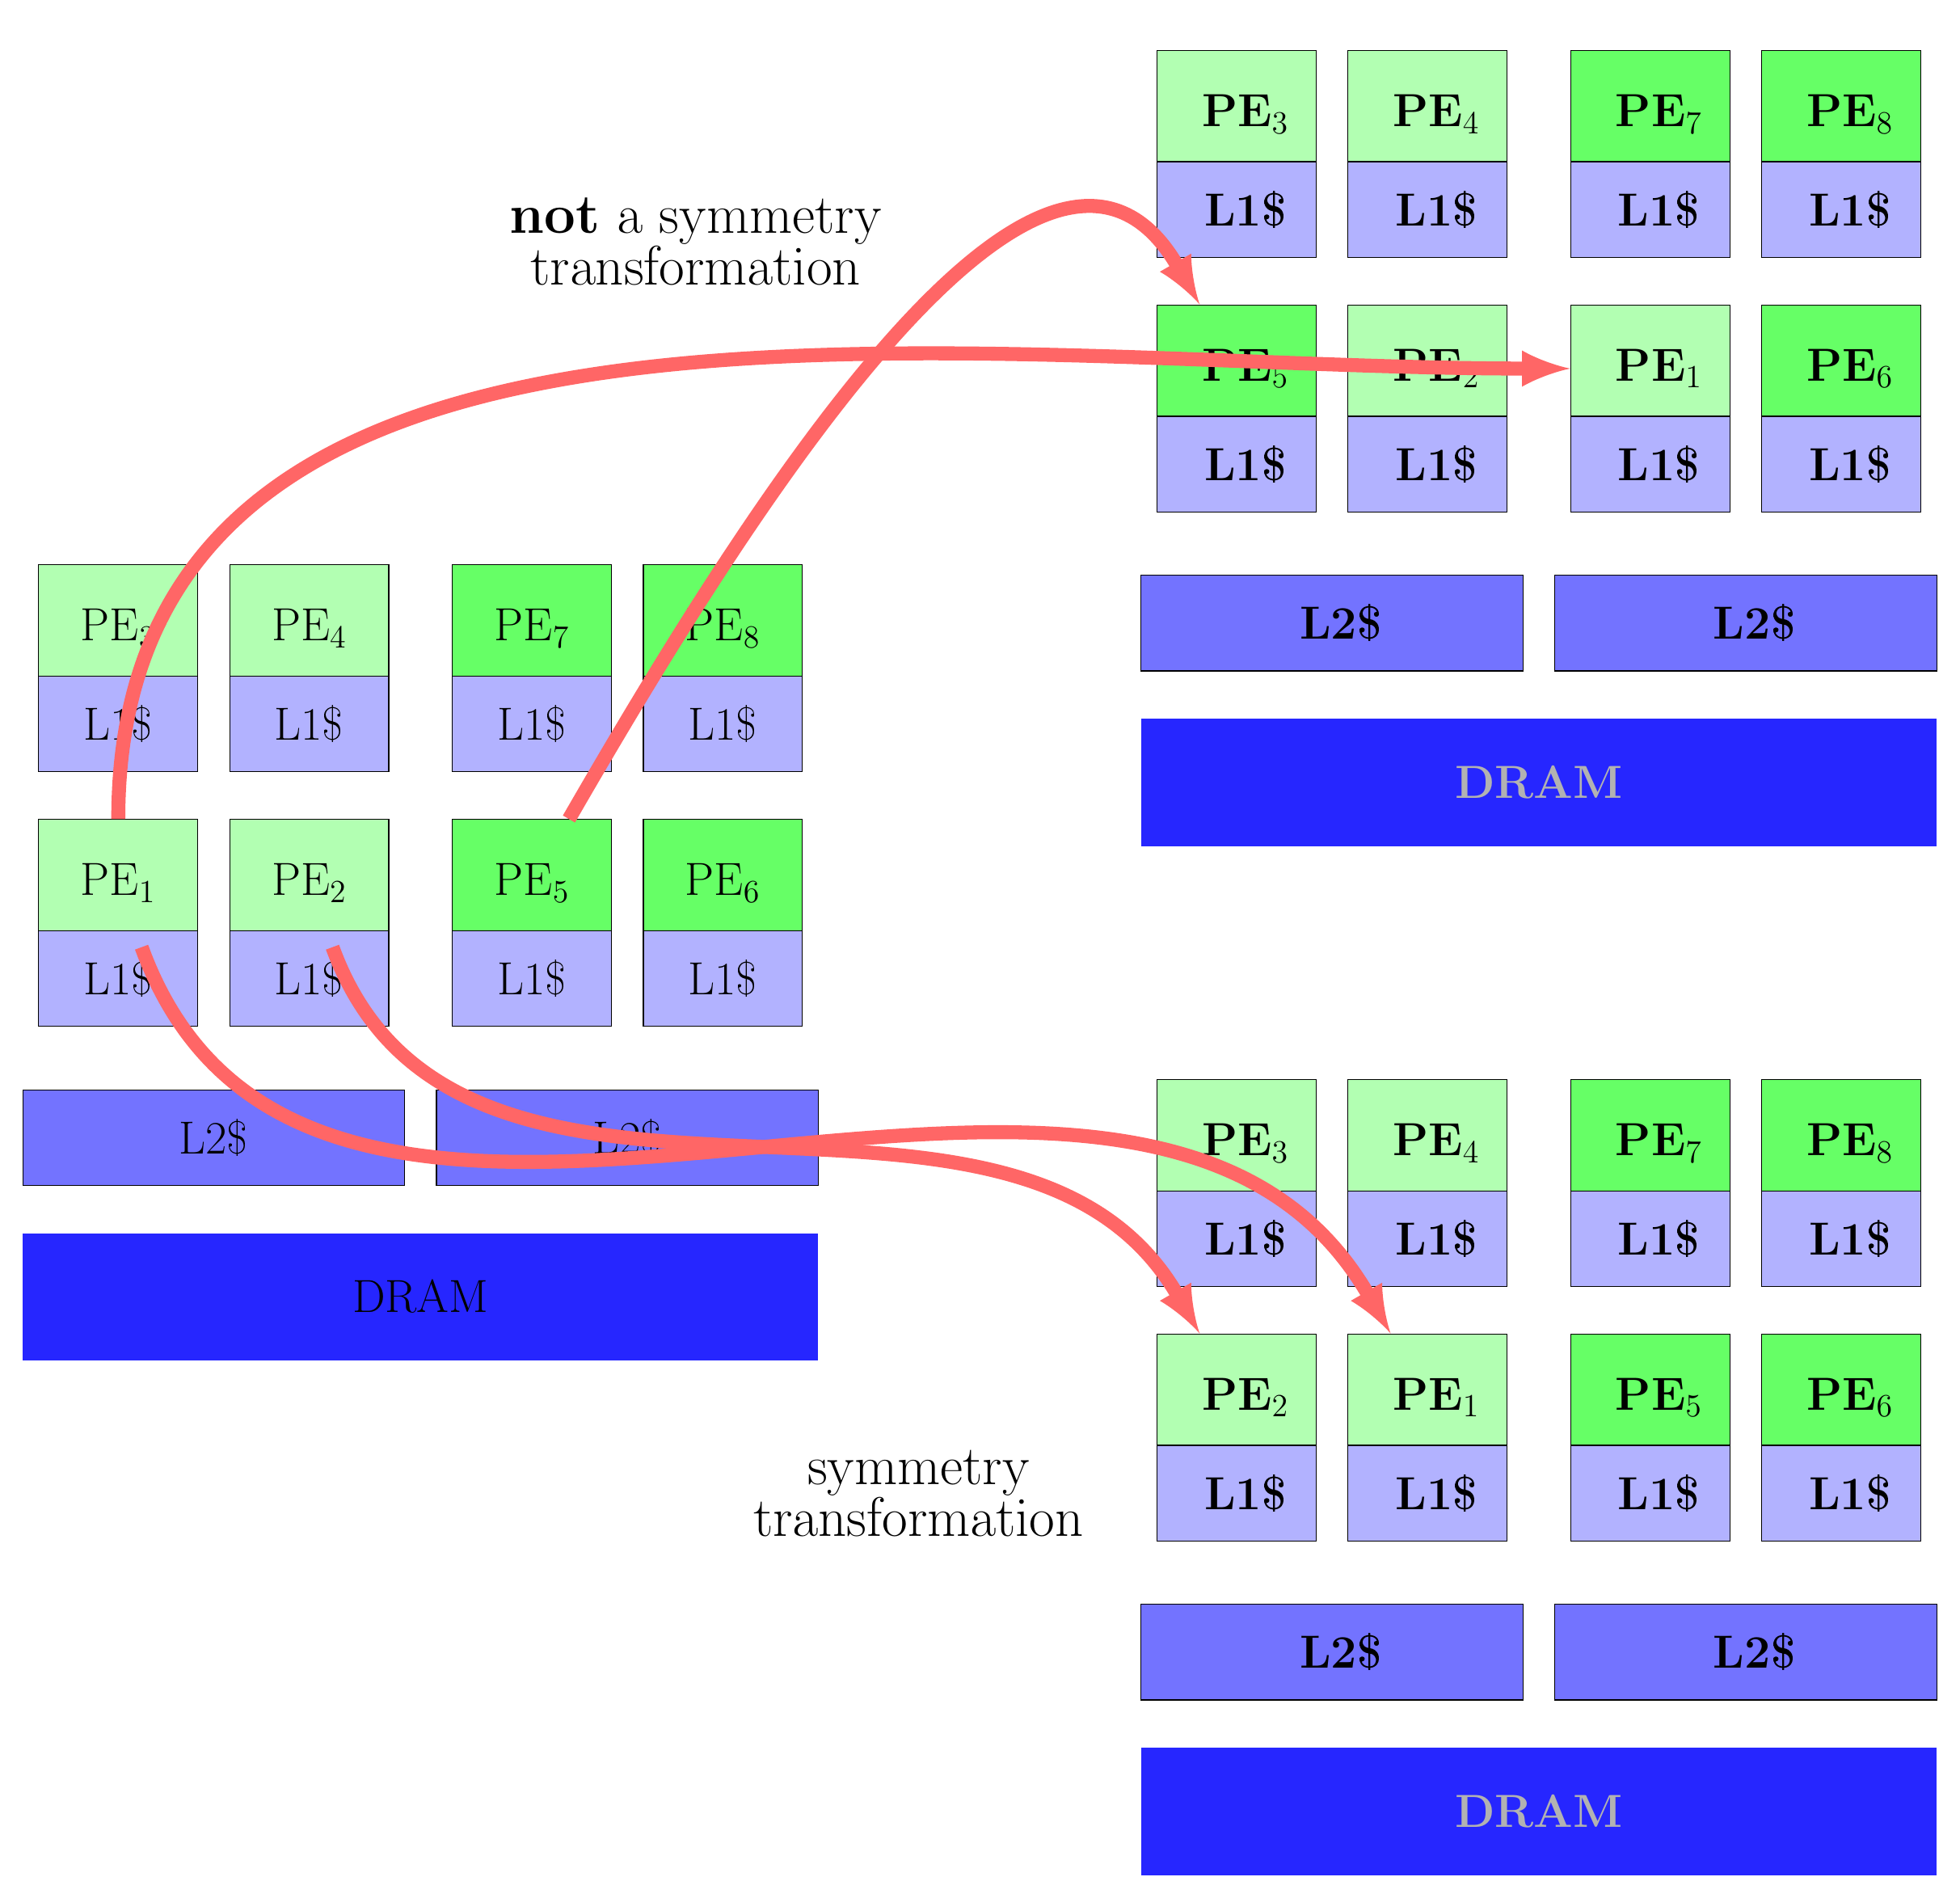
\begin{tikzpicture}
     \begin{scope}[name prefix=orig-]
%little cores
\node (pe1) at ({-1.5},{4}) [draw,minimum width=2.5cm,align=center,minimum height=2cm, fill=green!30] {\huge PE$_1$};
\node (L1-pe1) at (-1.5,2.5) [draw,minimum width=2.5cm,align=center,minimum height=1.5cm, fill=blue!30] {\huge L1\$};
\node (pe2) at (-1.5+3,4) [draw,minimum width=2.5cm,align=center,minimum height=2cm, fill=green!30] {\huge PE$_2$};
\node (L1-pe2) at (-1.5+3,2.5) [draw,minimum width=2.5cm,align=center,minimum height=1.5cm, fill=blue!30] {\huge L1\$};
\node (pe3) at (-1.5,4+4) [draw,minimum width=2.5cm,align=center,minimum height=2cm, fill=green!30] {\huge PE$_3$};
\node (L1-pe3) at (-1.5,2.5+4) [draw,minimum width=2.5cm,align=center,minimum height=1.5cm, fill=blue!30] {\huge L1\$};
\node (pe4) at (-1.5+3,4+4) [draw,minimum width=2.5cm,align=center,minimum height=2cm, fill=green!30] {\huge PE$_4$};
\node (L1-pe4) at (-1.5+3,2.5+4) [draw,minimum width=2.5cm,align=center,minimum height=1.5cm, fill=blue!30] {\huge L1\$};

%big cores
\node (pe5) at ({6.5-1.5},{4}) [draw,minimum width=2.5cm,align=center,minimum height=2cm, fill=green!60] {\huge PE$_5$};
\node (L1-pe5) at (6.5-1.5,2.5) [draw,minimum width=2.5cm,align=center,minimum height=1.5cm, fill=blue!30] {\huge L1\$};
\node (pe6) at (6.5-1.5+3,4) [draw,minimum width=2.5cm,align=center,minimum height=2cm, fill=green!60] {\huge PE$_6$};
\node (L1-pe6) at (6.5-1.5+3,2.5) [draw,minimum width=2.5cm,align=center,minimum height=1.5cm, fill=blue!30] {\huge L1\$};
\node (pe7) at (6.5-1.5,4+4) [draw,minimum width=2.5cm,align=center,minimum height=2cm, fill=green!60] {\huge PE$_7$};
\node (L1-pe7) at (6.5-1.5,2.5+4) [draw,minimum width=2.5cm,align=center,minimum height=1.5cm, fill=blue!30] {\huge L1\$};
\node (pe8) at (6.5-1.5+3,4+4) [draw,minimum width=2.5cm,align=center,minimum height=2cm, fill=green!60] {\huge PE$_8$};
\node (L1-pe8) at (6.5-1.5+3,2.5+4) [draw,minimum width=2.5cm,align=center,minimum height=1.5cm, fill=blue!30] {\huge L1\$};


\node (L2-little) at (0,0) [draw,minimum width=6cm,align=center,minimum height=1.5cm, fill=blue!55] {\huge L2\$};
\node (L2-big) at (6.5,0) [draw,minimum width=6cm,align=center,minimum height=1.5cm, fill=blue!55] {\huge L2\$};
\node (DRAM) at (3.25,-2.5) [minimum width=12.5cm,align=center,minimum height=2cm, fill=blue!85] {\huge DRAM};
\end{scope}

\begin{scope}[xshift=500, yshift=-230, name prefix=changed-]
%little cores
\node (pe2) at ({-1.5},{4}) [draw,minimum width=2.5cm,align=center,minimum height=2cm, fill=green!30] {\huge \textbf{ PE$_2$}};
\node (L1-pe2) at (-1.5,2.5) [draw,minimum width=2.5cm,align=center,minimum height=1.5cm, fill=blue!30] {\huge \textbf{ L1\$}};
\node (pe1) at (-1.5+3,4) [draw,minimum width=2.5cm,align=center,minimum height=2cm, fill=green!30] {\huge \textbf{ PE$_1$}};
\node (L1-pe1) at (-1.5+3,2.5) [draw,minimum width=2.5cm,align=center,minimum height=1.5cm, fill=blue!30] {\huge \textbf{ L1\$}};
\node (pe3) at (-1.5,4+4) [draw,minimum width=2.5cm,align=center,minimum height=2cm, fill=green!30] {\huge \textbf{ PE$_3$}};
\node (L1-pe3) at (-1.5,2.5+4) [draw,minimum width=2.5cm,align=center,minimum height=1.5cm, fill=blue!30] {\huge \textbf{ L1\$}};
\node (pe4) at (-1.5+3,4+4) [draw,minimum width=2.5cm,align=center,minimum height=2cm, fill=green!30] {\huge \textbf{ PE$_4$}};
\node (L1-pe4) at (-1.5+3,2.5+4) [draw,minimum width=2.5cm,align=center,minimum height=1.5cm, fill=blue!30] {\huge \textbf{ L1\$}};

%big cores
\node (pe5) at ({6.5-1.5},{4}) [draw,minimum width=2.5cm,align=center,minimum height=2cm, fill=green!60] {\huge \textbf{ PE$_5$}};
\node (L1-pe5) at (6.5-1.5,2.5) [draw,minimum width=2.5cm,align=center,minimum height=1.5cm, fill=blue!30] {\huge \textbf{ L1\$}};
\node (pe6) at (6.5-1.5+3,4) [draw,minimum width=2.5cm,align=center,minimum height=2cm, fill=green!60] {\huge \textbf{ PE$_6$}};
\node (L1-pe6) at (6.5-1.5+3,2.5) [draw,minimum width=2.5cm,align=center,minimum height=1.5cm, fill=blue!30] {\huge \textbf{ L1\$}};
\node (pe7) at (6.5-1.5,4+4) [draw,minimum width=2.5cm,align=center,minimum height=2cm, fill=green!60] {\huge \textbf{ PE$_7$}};
\node (L1-pe7) at (6.5-1.5,2.5+4) [draw,minimum width=2.5cm,align=center,minimum height=1.5cm, fill=blue!30] {\huge \textbf{ L1\$}};
\node (pe8) at (6.5-1.5+3,4+4) [draw,minimum width=2.5cm,align=center,minimum height=2cm, fill=green!60] {\huge \textbf{ PE$_8$}};
\node (L1-pe8) at (6.5-1.5+3,2.5+4) [draw,minimum width=2.5cm,align=center,minimum height=1.5cm, fill=blue!30] {\huge \textbf{ L1\$}};


\node (L2-little) at (0,0) [draw,minimum width=6cm,align=center,minimum height=1.5cm, fill=blue!55] {\huge \textbf{ L2\$}};
\node (L2-big) at (6.5,0) [draw,minimum width=6cm,align=center,minimum height=1.5cm, fill=blue!55] {\huge \textbf{ L2\$}};
\node (DRAM) at (3.25,-2.5) [minimum width=12.5cm,align=center,minimum height=2cm, fill=blue!85,text=black!30] {\huge \textbf{DRAM}};

\node (label) [align=center] at (-6.5,2.5) {\Huge symmetry \\ \Huge transformation};
\end{scope}

\draw (orig-pe1) edge[-{latex},line width=2.2mm, color=red!60,in=120,out=290,looseness=1]  (changed-pe1);
\draw (orig-pe2) edge[-{latex},line width=2.2mm, color=red!60,in=120,out=290,looseness=1]  (changed-pe2);


\begin{scope}[yshift=230, xshift=500,name prefix=non-]
%little cores
\node (pe5) at ({-1.5},{4}) [draw,minimum width=2.5cm,align=center,minimum height=2cm, fill=green!60] {\huge \textbf{ PE$_5$}};
\node (L1-pe5) at (-1.5,2.5) [draw,minimum width=2.5cm,align=center,minimum height=1.5cm, fill=blue!30] {\huge \textbf{ L1\$}};
\node (pe2) at (-1.5+3,4) [draw,minimum width=2.5cm,align=center,minimum height=2cm, fill=green!30] {\huge \textbf{ PE$_2$}};
\node (L1-pe2) at (-1.5+3,2.5) [draw,minimum width=2.5cm,align=center,minimum height=1.5cm, fill=blue!30] {\huge \textbf{ L1\$}};
\node (pe3) at (-1.5,4+4) [draw,minimum width=2.5cm,align=center,minimum height=2cm, fill=green!30] {\huge \textbf{ PE$_3$}};
\node (L1-pe3) at (-1.5,2.5+4) [draw,minimum width=2.5cm,align=center,minimum height=1.5cm, fill=blue!30] {\huge \textbf{ L1\$}};
\node (pe4) at (-1.5+3,4+4) [draw,minimum width=2.5cm,align=center,minimum height=2cm, fill=green!30] {\huge \textbf{ PE$_4$}};
\node (L1-pe4) at (-1.5+3,2.5+4) [draw,minimum width=2.5cm,align=center,minimum height=1.5cm, fill=blue!30] {\huge \textbf{ L1\$}};

%big cores
\node (pe1) at ({6.5-1.5},{4}) [draw,minimum width=2.5cm,align=center,minimum height=2cm, fill=green!30] {\huge \textbf{ PE$_1$}};
\node (L1-pe5) at (6.5-1.5,2.5) [draw,minimum width=2.5cm,align=center,minimum height=1.5cm, fill=blue!30] {\huge \textbf{ L1\$}};
\node (pe6) at (6.5-1.5+3,4) [draw,minimum width=2.5cm,align=center,minimum height=2cm, fill=green!60] {\huge \textbf{ PE$_6$}};
\node (L1-pe6) at (6.5-1.5+3,2.5) [draw,minimum width=2.5cm,align=center,minimum height=1.5cm, fill=blue!30] {\huge \textbf{ L1\$}};
\node (pe7) at (6.5-1.5,4+4) [draw,minimum width=2.5cm,align=center,minimum height=2cm, fill=green!60] {\huge \textbf{ PE$_7$}};
\node (L1-pe7) at (6.5-1.5,2.5+4) [draw,minimum width=2.5cm,align=center,minimum height=1.5cm, fill=blue!30] {\huge \textbf{ L1\$}};
\node (pe8) at (6.5-1.5+3,4+4) [draw,minimum width=2.5cm,align=center,minimum height=2cm, fill=green!60] {\huge \textbf{ PE$_8$}};
\node (L1-pe8) at (6.5-1.5+3,2.5+4) [draw,minimum width=2.5cm,align=center,minimum height=1.5cm, fill=blue!30] {\huge \textbf{ L1\$}};


\node (L2-little) at (0,0) [draw,minimum width=6cm,align=center,minimum height=1.5cm, fill=blue!55] {\huge \textbf{ L2\$}};
\node (L2-big) at (6.5,0) [draw,minimum width=6cm,align=center,minimum height=1.5cm, fill=blue!55] {\huge \textbf{ L2\$}};
\node (DRAM) at (3.25,-2.5) [minimum width=12.5cm,align=center,minimum height=2cm, fill=blue!85,text=black!30] {\huge \textbf{DRAM}};
\node (label) [align=center] at (-10,6) {\Huge \textbf{not} a symmetry \\ \Huge transformation};
\end{scope}

\draw (orig-pe1) edge[-{latex},line width=2.2mm, color=red!60,in=180,out=90,looseness=1]  (non-pe1);
\draw (orig-pe5) edge[-{latex},line width=2.2mm, color=red!60,in=120,out=60,looseness=1]  (non-pe5);
   \end{tikzpicture}
 }
   \caption{Examples of transformations in the Odroid-XU4 architecture.}
   \label{fig:exynos_symmetries}
\end{figure}

When the memory subsystem is more complex, this is also reflected in the topology. Consider the \ac{NoC}-based architecture depicted in the example, with four identical cores $\PE_1\ldots,\PE_4$.
An analogous transformation to the one described before, which swaps the cores $\PE_1$ and $\PE_2$, is not a symmetry of this topology, as depicted in Figure~\ref{fig:non_equivalent}.
The change in the cores changes the communication patterns.
Before the transformation, sending data from $\PE_1$ to $\PE_3$ needs two hops, whereas after the transformation it can be sent within a single hop, as shown by the red paths in the \ac{NoC}.

\begin{figure}[h]
	\centering
\resizebox{0.7\textwidth}{!}{
   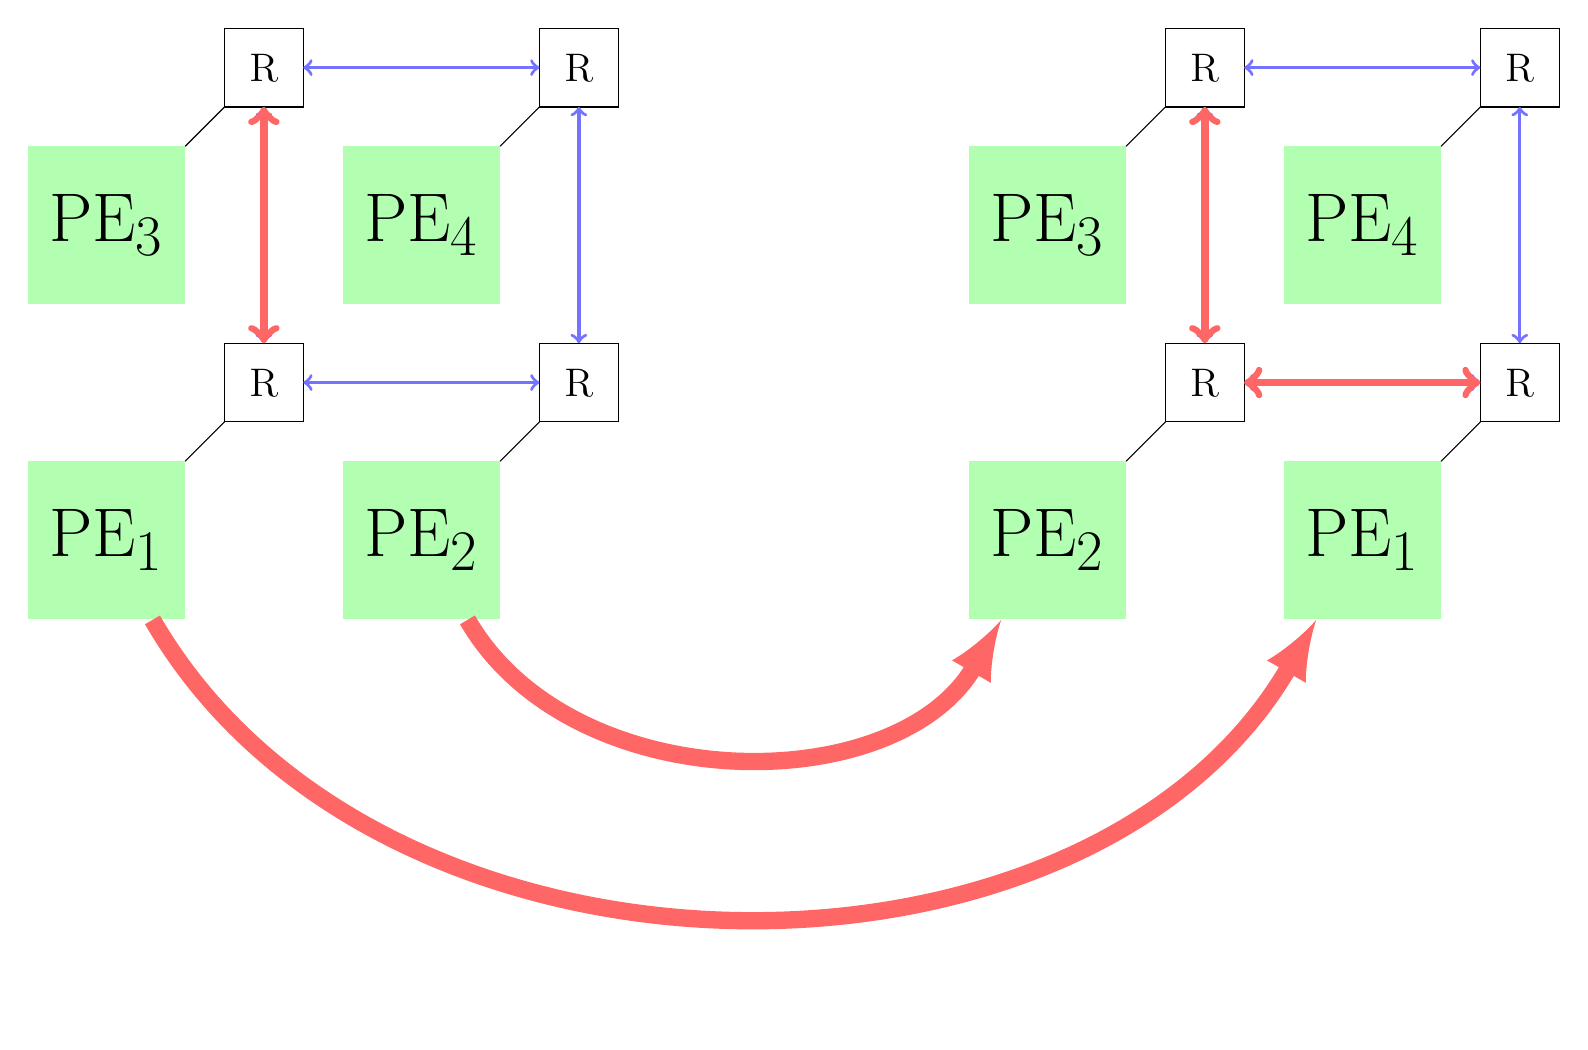
\begin{tikzpicture}
     
\begin{scope}[name prefix=orig-,xshift=-170]
  \node[rectangle,thick,minimum width = 2cm, minimum height=2cm,fill=green!30] (pe1) at (1,1) {\Huge PE$_1$};
  \node[rectangle,thick,minimum width = 2cm, minimum height=2cm,fill=green!30] (pe2) at (5,1) {\Huge PE$_2$};
  \node[rectangle,thick,minimum width = 2cm, minimum height=2cm,fill=green!30] (pe3) at (1,5) {\Huge PE$_3$};
  \node[rectangle,thick,minimum width = 2cm, minimum height=2cm,fill=green!30] (pe4) at (5,5) {\Huge PE$_4$};
  \foreach \x in {0,...,1}{
    \foreach \y in {0,...,1}{
       \pgfmathsetmacro{\xn}{\x*4}
       \pgfmathsetmacro{\yn}{\y*4} 
       \draw ({\xn + 2}, {\yn + 2}) -- ++(0.5,0.5);
       \draw ({\xn + 2.5},{\yn + 2.5}) rectangle ++(1,1) ++(-0.5,-0.5) node[font=\Large] {R};
      }
    }

  \foreach \x in {0,...,1}{
    \foreach \y in {0,...,1}{
      \pgfmathsetmacro{\xs}{\x*4+3}
      \pgfmathsetmacro{\ys}{\y*4+3}
      \pgfmathsetmacro{\xn}{\xs+3}
      \pgfmathsetmacro{\yn}{\ys+3}
      \pgfmathsetmacro{\xsm}{\x*4+3.5}
      \pgfmathsetmacro{\ysm}{\y*4+3.5}
      \pgfmathsetmacro{\xnm}{\xsm+3}
      \pgfmathsetmacro{\ynm}{\ysm+3}
      \ifnum\x<1
      \path[<->,very thick,blue!55] (\xsm,\ys) edge (\xnm,\ys);
      \fi
      \ifnum\y<1
      \path[<->,very thick,blue!55] (\xs,\ysm) edge (\xs,\ynm);
      \fi
      }
    }
      \path[<->,line width=1mm,red!60] (3,3.5) edge (3,6.5);

\end{scope}



\begin{scope}[name prefix=transformed-,xshift=170]
  \node[rectangle,thick,minimum width = 2cm, minimum height=2cm,fill=green!30] (pe2) at (1,1) {\Huge PE$_2$};
  \node[rectangle,thick,minimum width = 2cm, minimum height=2cm,fill=green!30] (pe1) at (5,1) {\Huge PE$_1$};
  \node[rectangle,thick,minimum width = 2cm, minimum height=2cm,fill=green!30] (pe3) at (1,5) {\Huge PE$_3$};
  \node[rectangle,thick,minimum width = 2cm, minimum height=2cm,fill=green!30] (pe4) at (5,5) {\Huge PE$_4$};
  \foreach \x in {0,...,1}{
    \foreach \y in {0,...,1}{
       \pgfmathsetmacro{\xn}{\x*4}
       \pgfmathsetmacro{\yn}{\y*4} 
       \draw ({\xn + 2}, {\yn + 2}) -- ++(0.5,0.5);
       \draw ({\xn + 2.5},{\yn + 2.5}) rectangle ++(1,1) ++(-0.5,-0.5) node[font=\Large] {R};
      }
    }

  \foreach \x in {0,...,1}{
    \foreach \y in {0,...,1}{
      \pgfmathsetmacro{\xs}{\x*4+3}
      \pgfmathsetmacro{\ys}{\y*4+3}
      \pgfmathsetmacro{\xn}{\xs+3}
      \pgfmathsetmacro{\yn}{\ys+3}
      \pgfmathsetmacro{\xsm}{\x*4+3.5}
      \pgfmathsetmacro{\ysm}{\y*4+3.5}
      \pgfmathsetmacro{\xnm}{\xsm+3}
      \pgfmathsetmacro{\ynm}{\ysm+3}
      \ifnum\x<1
      \path[<->,very thick,blue!55] (\xsm,\ys) edge (\xnm,\ys);
      \fi
      \ifnum\y<1
      \path[<->,very thick,blue!55] (\xs,\ysm) edge (\xs,\ynm);
      \fi
      }
    }

      \path[<->,line width=1mm,red!60] (3,3.5) edge (3,6.5);
      \path[<->,line width=1mm,red!60] (3.5,3) edge (6.5,3);

\end{scope}

\draw (orig-pe1) edge[-{latex},line width=2.2mm, color=red!60,in=240,out=300,looseness=1]  (transformed-pe1);
\draw (orig-pe2) edge[-{latex},line width=2.2mm, color=red!60,in=240,out=300,looseness=1]  (transformed-pe2);
   \end{tikzpicture}
 }
   \caption{The communication topology affects symmetries in architectures.}
   \label{fig:non_equivalent}
\end{figure}

Generally, the transformations that preserve the structure of the architecture topology have a clear structure.
If two transformations $t_1$ and $t_2$ preserve the structure of the architecture topology, then their composition $t_1 \circ t_2$ also preserves it.
Similarly, it is clear that reversing a transformation $t_1^{-1}$ also preserves the structure.
Finally, the identity transformation on the architecture $\operatorname{id}_A$ (which does not change anything) clearly preserves the structure.
These observations together mean that these transformations have the structure of a group with the function composition $(\circ)$ as its operation.

More precisely, the group of symmetries of the architecture is precisely the group of graph isomorphisms from the architecture graph $A$ to itself.
An isomorphism from an object to itself is called an automorphism\index{automorphism}.
We denote the group of automorphisms of the architecture $A$ as $\Aut(A)$

For the case of the \ac{NoC}-based architecture, the authomorphism group $\Aut(A_\text{NoC}) \cong D_4$ is a dihederal group on $4$ points.
It conists of $3$ rotations, $4$ reflections and the identity transformation.
The Odroid architecture, on the other hand, has $\Aut(A_\text{Odroid}) \cong S_4 \times S_4$ as symmetry group.
This group with $48$ transformations consists of (independent) arbitrary permutations of the A15 and A7 cores.

\begin{figure}[h]
	\centering
\resizebox{0.9\textwidth}{!}{
   \begin{tikzpicture}
     
\begin{scope}[xshift=0,yshift=0,scale=0.25]
\draw (15,1.25) node[rectangle, minimum height=300,minimum width=400,draw] (cluster1) {};
\tikzstyle{core} = [draw, text width=10em, minimum height=4em,
minimum width=4em, rounded corners, fill=gray!40, text centered]

%https://texample.net/tikz/examples/double-arrows/

\begin{scope}
\foreach \x in {15,14,...,1}{
  \node[core] (core_\x) at (\x,\x) {};
};
\node (core_0) [core] (0,0) {\Huge PE$_0$};
\end{scope}

\begin{scope}[xshift=800,yshift=80,scale=0.5]
\node (core_8) [core, fill=gray!60] (0,0) {\Huge Secure \& \\ Mngt. C.};
\end{scope}

\begin{scope}[xshift=400,yshift=-300]
  \draw[{Triangle[length=2mm,width=4.5mm]}-{Triangle[length=2mm,width=4.5mm]},line width=2.2mm ] (-15,2.5) -- (-15,7);
  \draw[{Triangle[length=2mm,width=4.5mm]}-{Triangle[length=2mm,width=4.5mm]},line width=2.2mm ] (15,2.5) -- (15,7);
  \node[draw,thick,text centered,minimum width=10cm,minimum height=10mm] (0,0) {\Huge SECURE BUS};
\end{scope}

\end{scope}

\begin{scope}[xshift=450,yshift=-350,scale=0.25]
\draw (15,1.25) node[rectangle, minimum height=300,minimum width=400,draw] (cluster2) {};
\tikzstyle{core} = [draw, text width=10em, minimum height=4em,
minimum width=4em, rounded corners, fill=gray!40, text centered]

%https://texample.net/tikz/examples/double-arrows/

\begin{scope}
\foreach \x in {15,14,...,1}{
  \node[core] (core_\x) at (\x,\x) {};
};
\node (core_0) [core] (0,0) {\Huge PE$_0$};
\end{scope}

\begin{scope}[xshift=800,yshift=80,scale=0.5]
\node (core_8) [core, fill=gray!60] (0,0) {\Huge Secure \& \\ Mngt. C.};
\end{scope}

\begin{scope}[xshift=400,yshift=-300]
  \draw[{Triangle[length=2mm,width=4.5mm]}-{Triangle[length=2mm,width=4.5mm]},line width=2.2mm ] (-15,2.5) -- (-15,7);
  \draw[{Triangle[length=2mm,width=4.5mm]}-{Triangle[length=2mm,width=4.5mm]},line width=2.2mm ] (15,2.5) -- (15,7);
  \node[draw,thick,text centered,minimum width=10cm,minimum height=10mm] (0,0) {\Huge SECURE BUS};
\end{scope}

\end{scope}

\begin{scope}[xshift=900,scale=0.25]
\draw (15,1.25) node[rectangle, minimum height=300,minimum width=400,draw] (cluster3) {};
\tikzstyle{core} = [draw, text width=10em, minimum height=4em,
minimum width=4em, rounded corners, fill=gray!40, text centered]

%https://texample.net/tikz/examples/double-arrows/

\begin{scope}
\foreach \x in {15,14,...,1}{
  \node[core] (core_\x) at (\x,\x) {};
};
\node (core_0) [core] (0,0) {\Huge PE$_0$};
\end{scope}

\begin{scope}[xshift=800,yshift=80,scale=0.5]
\node (core_8) [core, fill=gray!60] (0,0) {\Huge Secure \& \\ Mngt. C.};
\end{scope}

\begin{scope}[xshift=400,yshift=-300]
  \draw[{Triangle[length=2mm,width=4.5mm]}-{Triangle[length=2mm,width=4.5mm]},line width=2.2mm ] (-15,2.5) -- (-15,7);
  \draw[{Triangle[length=2mm,width=4.5mm]}-{Triangle[length=2mm,width=4.5mm]},line width=2.2mm ] (15,2.5) -- (15,7);
  \node[draw,thick,text centered,minimum width=10cm,minimum height=10mm] (0,0) {\Huge SECURE BUS};
\end{scope}

\end{scope}

\begin{scope}[xshift=200,yshift=400,scale=0.25]
\draw (15,1.25) node[rectangle, minimum height=300,minimum width=400,draw] (cluster4) {};
\tikzstyle{core} = [draw, text width=10em, minimum height=4em,
minimum width=4em, rounded corners, fill=gray!40, text centered]

%https://texample.net/tikz/examples/double-arrows/

\begin{scope}
\foreach \x in {15,14,...,1}{
  \node[core] (core_\x) at (\x,\x) {};
};
\node (core_0) [core] (0,0) {\Huge PE$_0$};
\end{scope}

\begin{scope}[xshift=800,yshift=80,scale=0.5]
\node (core_8) [core, fill=gray!60] (0,0) {\Huge Secure \& \\ Mngt. C.};
\end{scope}

\begin{scope}[xshift=400,yshift=-300]
  \draw[{Triangle[length=2mm,width=4.5mm]}-{Triangle[length=2mm,width=4.5mm]},line width=2.2mm ] (-15,2.5) -- (-15,7);
  \draw[{Triangle[length=2mm,width=4.5mm]}-{Triangle[length=2mm,width=4.5mm]},line width=2.2mm ] (15,2.5) -- (15,7);
  \node[draw,thick,text centered,minimum width=10cm,minimum height=10mm] (0,0) {\Huge SECURE BUS};
\end{scope}

\end{scope}

\begin{scope}[xshift=700,yshift=400,scale=0.25]
\draw (15,1.25) node[rectangle, minimum height=300,minimum width=400,draw] (cluster5) {};
\tikzstyle{core} = [draw, text width=10em, minimum height=4em,
minimum width=4em, rounded corners, fill=gray!40, text centered]

%https://texample.net/tikz/examples/double-arrows/

\begin{scope}
\foreach \x in {15,14,...,1}{
  \node[core] (core_\x) at (\x,\x) {};
};
\node (core_0) [core] (0,0) {\Huge PE$_0$};
\end{scope}

\begin{scope}[xshift=800,yshift=80,scale=0.5]
\node (core_8) [core, fill=gray!60] (0,0) {\Huge Secure \& \\ Mngt. C.};
\end{scope}

\begin{scope}[xshift=400,yshift=-300]
  \draw[{Triangle[length=2mm,width=4.5mm]}-{Triangle[length=2mm,width=4.5mm]},line width=2.2mm ] (-15,2.5) -- (-15,7);
  \draw[{Triangle[length=2mm,width=4.5mm]}-{Triangle[length=2mm,width=4.5mm]},line width=2.2mm ] (15,2.5) -- (15,7);
  \node[draw,thick,text centered,minimum width=10cm,minimum height=10mm] (0,0) {\Huge SECURE BUS};
\end{scope}

\end{scope}


\draw [latex-latex,line width=1.1mm] (cluster1) -- (cluster2); 
\draw [latex-latex,line width=1.1mm] (cluster1) -- (cluster3); 
\draw [latex-latex,line width=1.1mm] (cluster1) -- (cluster4); 
\draw [latex-latex,line width=1.1mm] (cluster1) -- (cluster5); 
\draw [latex-latex,line width=1.1mm] (cluster2) -- (cluster3); 
\draw [latex-latex,line width=1.1mm] (cluster2) -- (cluster4); 
\draw [latex-latex,line width=1.1mm] (cluster2) -- (cluster5); 
\draw [latex-latex,line width=1.1mm] (cluster3) -- (cluster4); 
\draw [latex-latex,line width=1.1mm] (cluster3) -- (cluster5); 
\draw [latex-latex,line width=1.1mm] (cluster4) -- (cluster5); 
   \end{tikzpicture}
 }
   \caption{The topology of the Kalray MPPA3 Coolidge.}
   \label{fig:coolidge}
\end{figure}

Since the Odroid architecture is heterogeneous, both clusters are distinct and there is no symmetry between them.
Many complex architectures, however, do consist of multiple identical clusters.
Consider the architecture depicted in Figure~\ref{fig:coolidge}.
It is the MPPA3 Coolidge from Kalray~\cite{coolidge} and consists of $5$ identical clusters.
Each cluster has $17$ cores, $16$ of which are identical general-purpose cores, and the last one is a special-purpose secure and management core.

The MPPA3 Coolidge is a hierarchically-designed architecture. The five identical clusters are conceptually at a different level than the cores at each cluster.
Designs like the HAEC~\cite{HAEC} topology mentioned in the introduction (cf. Figure~\ref{fig:haec}) have even more levels of hierarchy.
The symmetries of these hierarchical architectures are reflected in the different levels of hierarchy of the topology~\cite{goens_tcad21}.
For example, the automorphism group of the MPPA3 Coolidge is $\Aut(A_\text{Coolidge}) \cong S_{16} \wr S_5$ and has $16! \cdot 5! \approx 2.51 \cdot 10^{15}$ symmetries. 

So far we have discussed the symmetries of architectures.
However, we can apply the same principle to applications and their graphs.
Conisder the audio filter example application from Section~\ref{sec:kpn_basic} (cf. Figure~\ref{fig:audio_filter_graph}). 
The left and right channels perform precisely the same computation on different data.
We could not, for example, just swap the \texttt{fft\_l} and \texttt{fft\_r} nodes, since that would result in a different application that also swaps the channels of the audio file.
On the other hand, if we swap the whole subgraph consisting of \texttt{fft\_l}, \texttt{filter\_l} and \texttt{ifft\_l} with the equivalent subgraph of \texttt{fft\_r}, \texttt{filter\_r} and \texttt{ifft\_r}, the application remains identical.
This is depicted on Figure~\ref{fig:audio_filter_symmetries}.

\begin{figure}[h]
	\centering
\resizebox{0.9\textwidth}{!}{
\begin{tikzpicture}
   \begin{scope}[name prefix=orig-]
\node[draw, ellipse,minimum width = 1.1cm, minimum height=0.9cm] (src) {src};
\node[draw, ellipse,minimum width = 1.1cm, minimum height=0.9cm, below right = 1cm of src] (fft_l) {\texttt{fft\_l}};
\node[draw, ellipse,minimum width = 1.1cm, minimum height=0.9cm, above right = 1cm of src] (fft_r) {\texttt{fft\_r}};
\node[draw, ellipse,minimum width = 1.1cm, minimum height=0.9cm, right = 1 cm of fft_l] (filter_l) {\texttt{filter\_l}};
\node[draw, ellipse,minimum width = 1.1cm, minimum height=0.9cm, right = 1 cm of fft_r] (filter_r) {\texttt{filter\_r}};
\node[draw, ellipse,minimum width = 1.1cm, minimum height=0.9cm, right = 1 cm of filter_l] (ifft_l) {\texttt{ifft\_l}};
\node[draw, ellipse,minimum width = 1.1cm, minimum height=0.9cm, right = 1 cm of filter_r] (ifft_r) {\texttt{ifft\_r}};
\node[draw, ellipse,minimum width = 1.1cm, minimum height=0.9cm, below right = 1cm of ifft_r] (sink) {\texttt{sink}};

\draw[-latex] (src) -- (fft_l);
\draw[-latex] (src) -- (fft_r);
\draw[-latex] (fft_l) -- (filter_l);
\draw[-latex] (fft_r) -- (filter_r);
\draw[-latex] (filter_l) -- (ifft_l);
\draw[-latex] (filter_r) -- (ifft_r);
\draw[-latex] (ifft_l) -- (sink);
\draw[-latex] (ifft_r) -- (sink);

\node (label) [align=center] at (12,0) { \large original};
\end{scope}

\begin{scope}[name prefix=transformed-,xshift=140,yshift=-140]
\node[draw, ellipse,minimum width = 1.1cm, minimum height=0.9cm] (src) {\texttt{src}};
\node[draw, ellipse,minimum width = 1.1cm, minimum height=0.9cm, below right = 1cm of src] (fft_r) {\texttt{fft\_r}};
\node[draw, ellipse,minimum width = 1.1cm, minimum height=0.9cm, above right = 1cm of src] (fft_l) {\texttt{fft\_l}};
\node[draw, ellipse,minimum width = 1.1cm, minimum height=0.9cm, right = 1 cm of fft_r] (filter_r) {\texttt{filter\_r}};
\node[draw, ellipse,minimum width = 1.1cm, minimum height=0.9cm, right = 1 cm of fft_l] (filter_l) {\texttt{filter\_l}};
\node[draw, ellipse,minimum width = 1.1cm, minimum height=0.9cm, right = 1 cm of filter_r] (ifft_r) {\texttt{ifft\_r}};
\node[draw, ellipse,minimum width = 1.1cm, minimum height=0.9cm, right = 1 cm of filter_l] (ifft_l) {\texttt{ifft\_l}};
\node[draw, ellipse,minimum width = 1.1cm, minimum height=0.9cm, below right = 1cm of ifft_l] (sink) {\texttt{sink}};

\draw[-latex] (src) -- (fft_l);
\draw[-latex] (src) -- (fft_r);
\draw[-latex] (fft_l) -- (filter_l);
\draw[-latex] (fft_r) -- (filter_r);
\draw[-latex] (filter_l) -- (ifft_l);
\draw[-latex] (filter_r) -- (ifft_r);
\draw[-latex] (ifft_l) -- (sink);
\draw[-latex] (ifft_r) -- (sink);

\node (label) [align=center] at (-3.5,0) {\large transformed};
\end{scope}


\draw (orig-fft_l) edge[-{latex},line width=1.2mm, color=red!60,in=140,out=310,looseness=1]  (transformed-fft_l);
\draw (orig-ifft_l) edge[-{latex},line width=1.2mm, color=red!60,in=140,out=310,looseness=1]  (transformed-ifft_l);
\draw (orig-filter_l) edge[-{latex},line width=1.2mm, color=red!60,in=140,out=310,looseness=1]  (transformed-filter_l);
\draw (orig-fft_r) edge[-{latex},line width=1.2mm, color=red!60,in=120,out=290,looseness=1]  (transformed-fft_r);
\draw (orig-ifft_r) edge[-{latex},line width=1.2mm, color=red!60,in=120,out=290,looseness=1]  (transformed-ifft_r);
\draw (orig-filter_r) edge[-{latex},line width=1.2mm, color=red!60,in=120,out=290,looseness=1]  (transformed-filter_r);
 \end{tikzpicture}
}
   \caption{A symmetry transformation of the audio filter application.}
	\label{fig:audio_filter_symmetries}
\end{figure}

Mathematically, we need to model the semantics of the application to reflect its symmetries.
For an application $K = (V_K,E_K)$ we can label the nodes $V_K$ with unique identifiers relating them to the $KPN$ process that execute them (e.g. the \texttt{\_\_PNprocess} in a \ac{CPN} program). 
Formally, thus, the automorphism group $\Aut(E)$ of the labeled graph $K$ is trivial, i.e. $\Aut(E) = \{ \id \}$. 
We could label $K$ differently to capture the symmetry from Figure~\ref{fig:audio_filter_symmetries}.
For example, if use the source code of the process as label, we would capture this symmetry.
We have to be careful, however, as this can lead to a problematic definition of symmetries.

An application might use the same code at different points, resulting in very different behavior.
For example, consider an application that receives a list of points, which it sorts before operating on it.
Before returning the list, it sorts them again to ensure they are sorted.
Both times it sorts the list using the quicksort algorithm, yet the second time the list is almost always sorted or close to being sorted.
Then, the execution of the same quicksort code in the second instance behaves very differently from the first time.

A difference like the one outlined above is very difficult to capture automatically, as it requires understanding of the application to a very high level of abstraction.
We thus consider application symmetries as manually-defined annotations.
There are some conceivable ways to automatically capture and annotate such application symmetries, for example when dealing with known \ac{DLP}.
In future work, a framework as we discuss in Chapter~\ref{chap:mocs}, Section~\ref{sec:macqueen} could be extended to extract application symmetries from \ac{DLP}.
For the rest of this thesis, however, we focus on symmetries induced from the architecture.

\subsection{Mappings}

We have seen how the architecture and applications have symmetries in their structure. 
The groups $\Aut(A)$ and $\Aut(K)$ act on the architecture $A$ and the application $K$, respectively.
These actions also induce an action on the mapping space. 
Let $m : K \rightarrow A$ be a mapping.
Recall that a symmetry $\sigma \in \Aut(A)$ of the architecture is a transformation that leaves the structure of the architecture unchanged.
Conisder then the mapping $\sigma m := k \mapsto \sigma(m(k))$.
Since the structure of $A$ is unchanged, then the structure of $m$ and $\sigma m$ is also identical.
All observable properties $\Theta$ of $m$ and $\sigma m$, like the execution time or energy consumption, are the same.
If they were not, it would have to be due to a structural difference in the (sub)architectures $m(K),(\sigma m)(k) = \sigma(m(K)) \leq A$, which are isomorphic by assumption on $\sigma$.
We say that these properties like the execution time and energy consumption are \emph{invariants}\index{invariants} of the group action.

The case for $K$ is analogous.
Let $\pi \in \Aut(K)$ be a symmetry of the application.
Then the mapping $\pi m := k \mapsto m(\pi^{-1}k)$ is equivalent to $m$.
Note that we define it with $\pi^{-1}$ instead of $\pi$ so that this defines a left action.
Indeed, for $\pi, \tau \in \Aut(K)$, we have
\begin{align*}
  (\pi (\tau m))(k) = \pi m(\tau^{-1}k) = m(\pi^{-1}\tau^{-1}k) = m((\tau \pi)^{-1}k) = ((\tau \pi) m))(k) 
\end{align*}

\begin{figure}[h]
	\centering
\resizebox{1.0\textwidth}{!}{
\begin{tikzpicture}
   \begin{scope}[xshift=-500,yshift=113,scale=2,every node/.style={scale=2}]
\node[draw, ellipse,minimum width = 1.1cm, minimum height=0.9cm] (src) {t$_1$};
\node[draw, ellipse,minimum width = 1.1cm, minimum height=0.9cm, below right = 1cm of src] (fft_l) {t$_2$};
\node[draw, ellipse,minimum width = 1.1cm, minimum height=0.9cm, above right = 1cm of src] (fft_r) {t$_3$};
\node[draw, ellipse,minimum width = 1.1cm, minimum height=0.9cm, right = 1 cm of fft_l] (filter_l) {t$_4$};
\node[draw, ellipse,minimum width = 1.1cm, minimum height=0.9cm, right = 1 cm of fft_r] (filter_r) {t$_5$};
\node[draw, ellipse,minimum width = 1.1cm, minimum height=0.9cm, right = 1 cm of filter_l] (ifft_l) {t$_6$};
\node[draw, ellipse,minimum width = 1.1cm, minimum height=0.9cm, right = 1 cm of filter_r] (ifft_r) {t$_7$};
\node[draw, ellipse,minimum width = 1.1cm, minimum height=0.9cm, below right = 1cm of ifft_r] (sink) {t$_8$};
\draw[-latex] (src) -- (fft_l);
\draw[-latex] (src) -- (fft_r);
\draw[-latex] (fft_l) -- (filter_l);
\draw[-latex] (fft_r) -- (filter_r);
\draw[-latex] (filter_l) -- (ifft_l);
\draw[-latex] (filter_r) -- (ifft_r);
\draw[-latex] (ifft_l) -- (sink);
\draw[-latex] (ifft_r) -- (sink);
\end{scope}


\begin{scope}[name prefix=orig-]
%little cores
\node (pe1) at ({-1.5},{4}) [draw,minimum width=2.5cm,align=center,minimum height=2cm, fill=green!30] {\huge PE$_1$};
\node (L1-pe1) at (-1.5,2.5) [draw,minimum width=2.5cm,align=center,minimum height=1.5cm, fill=blue!30] {\huge L1\$};
\node (pe2) at (-1.5+3,4) [draw,minimum width=2.5cm,align=center,minimum height=2cm, fill=green!30] {\huge PE$_2$};
\node (L1-pe2) at (-1.5+3,2.5) [draw,minimum width=2.5cm,align=center,minimum height=1.5cm, fill=blue!30] {\huge L1\$};
\node (pe3) at (-1.5,4+4) [draw,minimum width=2.5cm,align=center,minimum height=2cm, fill=green!30] {\huge PE$_3$};
\node (L1-pe3) at (-1.5,2.5+4) [draw,minimum width=2.5cm,align=center,minimum height=1.5cm, fill=blue!30] {\huge L1\$};
\node (pe4) at (-1.5+3,4+4) [draw,minimum width=2.5cm,align=center,minimum height=2cm, fill=green!30] {\huge PE$_4$};
\node (L1-pe4) at (-1.5+3,2.5+4) [draw,minimum width=2.5cm,align=center,minimum height=1.5cm, fill=blue!30] {\huge L1\$};

%big cores
\node (pe5) at ({6.5-1.5},{4}) [draw,minimum width=2.5cm,align=center,minimum height=2cm, fill=green!60] {\huge PE$_5$};
\node (L1-pe5) at (6.5-1.5,2.5) [draw,minimum width=2.5cm,align=center,minimum height=1.5cm, fill=blue!30] {\huge L1\$};
\node (pe6) at (6.5-1.5+3,4) [draw,minimum width=2.5cm,align=center,minimum height=2cm, fill=green!60] {\huge PE$_6$};
\node (L1-pe6) at (6.5-1.5+3,2.5) [draw,minimum width=2.5cm,align=center,minimum height=1.5cm, fill=blue!30] {\huge L1\$};
\node (pe7) at (6.5-1.5,4+4) [draw,minimum width=2.5cm,align=center,minimum height=2cm, fill=green!60] {\huge PE$_7$};
\node (L1-pe7) at (6.5-1.5,2.5+4) [draw,minimum width=2.5cm,align=center,minimum height=1.5cm, fill=blue!30] {\huge L1\$};
\node (pe8) at (6.5-1.5+3,4+4) [draw,minimum width=2.5cm,align=center,minimum height=2cm, fill=green!60] {\huge PE$_8$};
\node (L1-pe8) at (6.5-1.5+3,2.5+4) [draw,minimum width=2.5cm,align=center,minimum height=1.5cm, fill=blue!30] {\huge L1\$};


\node (L2-little) at (0,0) [draw,minimum width=6cm,align=center,minimum height=1.5cm, fill=blue!55] {\huge L2\$};
\node (L2-big) at (6.5,0) [draw,minimum width=6cm,align=center,minimum height=1.5cm, fill=blue!55] {\huge L2\$};
\node (DRAM) at (3.25,-2.5) [minimum width=12.5cm,align=center,minimum height=2cm, fill=blue!85] {\huge DRAM};
\node[ellipse,fill=red!60] (t1) at (pe2) {\Huge t$_1$};
\node[ellipse,fill=red!60,anchor=north west] (t2) at (pe1.north west) {\Huge t$_2$};
\node[ellipse,fill=red!60] (t3) at (pe1) {\Huge t$_3$};
\node[ellipse,fill=red!60,anchor=north west] (t4) at (pe5.north west) {\Huge t$_4$};
\node[ellipse,fill=red!60,anchor=south east] (t5) at (pe1.south east) {\Huge t$_5$};
\node[ellipse,fill=red!60,anchor=south east] (t6) at (pe5.south east) {\Huge t$_6$};
\node[ellipse,fill=red!60] (t7) at (pe3) {\Huge t$_7$};
\node[ellipse,fill=red!60] (t8) at (pe7) {\Huge t$_8$};
\end{scope}


\draw[-{Triangle[length=4mm,width=9.5mm]},line width=6.2mm,color=black!20,shorten >= 3mm, shorten <=3mm] (sink) -- (orig-pe1);

\begin{scope}[xshift=500, yshift=-230, name prefix=arch-]
%little cores
\node (pe1) at ({-1.5},{4}) [draw,minimum width=2.5cm,align=center,minimum height=2cm, fill=green!30] {\huge PE$_1$};
\node (L1-pe1) at (-1.5,2.5) [draw,minimum width=2.5cm,align=center,minimum height=1.5cm, fill=blue!30] {\huge L1\$};
\node (pe2) at (-1.5+3,4) [draw,minimum width=2.5cm,align=center,minimum height=2cm, fill=green!30] {\huge PE$_2$};
\node (L1-pe2) at (-1.5+3,2.5) [draw,minimum width=2.5cm,align=center,minimum height=1.5cm, fill=blue!30] {\huge L1\$};
\node (pe3) at (-1.5,4+4) [draw,minimum width=2.5cm,align=center,minimum height=2cm, fill=green!30] {\huge PE$_3$};
\node (L1-pe3) at (-1.5,2.5+4) [draw,minimum width=2.5cm,align=center,minimum height=1.5cm, fill=blue!30] {\huge L1\$};
\node (pe4) at (-1.5+3,4+4) [draw,minimum width=2.5cm,align=center,minimum height=2cm, fill=green!30] {\huge PE$_4$};
\node (L1-pe4) at (-1.5+3,2.5+4) [draw,minimum width=2.5cm,align=center,minimum height=1.5cm, fill=blue!30] {\huge L1\$};

%big cores
\node (pe5) at ({6.5-1.5},{4}) [draw,minimum width=2.5cm,align=center,minimum height=2cm, fill=green!60] {\huge PE$_5$};
\node (L1-pe5) at (6.5-1.5,2.5) [draw,minimum width=2.5cm,align=center,minimum height=1.5cm, fill=blue!30] {\huge L1\$};
\node (pe6) at (6.5-1.5+3,4) [draw,minimum width=2.5cm,align=center,minimum height=2cm, fill=green!60] {\huge PE$_6$};
\node (L1-pe6) at (6.5-1.5+3,2.5) [draw,minimum width=2.5cm,align=center,minimum height=1.5cm, fill=blue!30] {\huge L1\$};
\node (pe7) at (6.5-1.5,4+4) [draw,minimum width=2.5cm,align=center,minimum height=2cm, fill=green!60] {\huge PE$_7$};
\node (L1-pe7) at (6.5-1.5,2.5+4) [draw,minimum width=2.5cm,align=center,minimum height=1.5cm, fill=blue!30] {\huge L1\$};
\node (pe8) at (6.5-1.5+3,4+4) [draw,minimum width=2.5cm,align=center,minimum height=2cm, fill=green!60] {\huge PE$_8$};
\node (L1-pe8) at (6.5-1.5+3,2.5+4) [draw,minimum width=2.5cm,align=center,minimum height=1.5cm, fill=blue!30] {\huge L1\$};


\node (L2-little) at (0,0) [draw,minimum width=6cm,align=center,minimum height=1.5cm, fill=blue!55] {\huge L2\$};
\node (L2-big) at (6.5,0) [draw,minimum width=6cm,align=center,minimum height=1.5cm, fill=blue!55] {\huge L2\$};
\node (DRAM) at (3.25,-2.5) [minimum width=12.5cm,align=center,minimum height=2cm, fill=blue!85] {\huge DRAM};

\node (label) [align=center] at (-8.5,2.5) {\Huge architecture symmetry: \\ \Huge (PE$_1$,PE$_2$)};
\node[ellipse,fill=red!60] (t1) at (pe1) {\Huge t$_1$};
\node[ellipse,fill=red!60,anchor=north west] (t2) at (pe2.north west) {\Huge t$_2$};
\node[ellipse,fill=red!60] (t3) at (pe2) {\Huge t$_3$};
\node[ellipse,fill=red!60,anchor=north west] (t4) at (pe5.north west) {\Huge t$_4$};
\node[ellipse,fill=red!60,anchor=south east] (t5) at (pe2.south east) {\Huge t$_5$};
\node[ellipse,fill=red!60,anchor=south east] (t6) at (pe5.south east) {\Huge t$_6$};
\node[ellipse,fill=red!60] (t7) at (pe3) {\Huge t$_7$};
\node[ellipse,fill=red!60] (t8) at (pe7) {\Huge t$_8$};

\end{scope}


\begin{scope}[yshift=230, xshift=500,name prefix=app-]
%little cores
\node (pe1) at ({-1.5},{4}) [draw,minimum width=2.5cm,align=center,minimum height=2cm, fill=green!30] {\huge PE$_1$};
\node (L1-pe1) at (-1.5,2.5) [draw,minimum width=2.5cm,align=center,minimum height=1.5cm, fill=blue!30] {\huge L1\$};
\node (pe2) at (-1.5+3,4) [draw,minimum width=2.5cm,align=center,minimum height=2cm, fill=green!30] {\huge PE$_2$};
\node (L1-pe2) at (-1.5+3,2.5) [draw,minimum width=2.5cm,align=center,minimum height=1.5cm, fill=blue!30] {\huge L1\$};
\node (pe3) at (-1.5,4+4) [draw,minimum width=2.5cm,align=center,minimum height=2cm, fill=green!30] {\huge PE$_3$};
\node (L1-pe3) at (-1.5,2.5+4) [draw,minimum width=2.5cm,align=center,minimum height=1.5cm, fill=blue!30] {\huge L1\$};
\node (pe4) at (-1.5+3,4+4) [draw,minimum width=2.5cm,align=center,minimum height=2cm, fill=green!30] {\huge PE$_4$};
\node (L1-pe4) at (-1.5+3,2.5+4) [draw,minimum width=2.5cm,align=center,minimum height=1.5cm, fill=blue!30] {\huge L1\$};

%big cores
\node (pe5) at ({6.5-1.5},{4}) [draw,minimum width=2.5cm,align=center,minimum height=2cm, fill=green!60] {\huge PE$_5$};
\node (L1-pe5) at (6.5-1.5,2.5) [draw,minimum width=2.5cm,align=center,minimum height=1.5cm, fill=blue!30] {\huge L1\$};
\node (pe6) at (6.5-1.5+3,4) [draw,minimum width=2.5cm,align=center,minimum height=2cm, fill=green!60] {\huge PE$_6$};
\node (L1-pe6) at (6.5-1.5+3,2.5) [draw,minimum width=2.5cm,align=center,minimum height=1.5cm, fill=blue!30] {\huge L1\$};
\node (pe7) at (6.5-1.5,4+4) [draw,minimum width=2.5cm,align=center,minimum height=2cm, fill=green!60] {\huge PE$_7$};
\node (L1-pe7) at (6.5-1.5,2.5+4) [draw,minimum width=2.5cm,align=center,minimum height=1.5cm, fill=blue!30] {\huge L1\$};
\node (pe8) at (6.5-1.5+3,4+4) [draw,minimum width=2.5cm,align=center,minimum height=2cm, fill=green!60] {\huge PE$_8$};
\node (L1-pe8) at (6.5-1.5+3,2.5+4) [draw,minimum width=2.5cm,align=center,minimum height=1.5cm, fill=blue!30] {\huge L1\$};


\node (L2-little) at (0,0) [draw,minimum width=6cm,align=center,minimum height=1.5cm, fill=blue!55] {\huge L2\$};
\node (L2-big) at (6.5,0) [draw,minimum width=6cm,align=center,minimum height=1.5cm, fill=blue!55] {\huge L2\$};
\node (DRAM) at (3.25,-2.5) [minimum width=12.5cm,align=center,minimum height=2cm, fill=blue!85] {\huge DRAM};
\node (label) [align=center] at (-11,6) {\Huge  application symmetry: \\ \Huge (t$_2$,t$_3$)(t$_4$,t$_5$)(t$_6$,t$_7$)};
\node[ellipse,fill=red!60] (t1) at (pe2) {\Huge t$_1$};
\node[ellipse,fill=red!60] (t2) at (pe1) {\Huge t$_2$};
\node[ellipse,fill=red!60,anchor=north west] (t3) at (pe1.north west) {\Huge t$_3$};
\node[ellipse,fill=red!60,anchor=south east] (t4) at (pe1.south east) {\Huge t$_4$};
\node[ellipse,fill=red!60,anchor=north west] (t5) at (pe5.north west) {\Huge t$_5$};
\node[ellipse,fill=red!60] (t6) at (pe3) {\Huge t$_6$};
\node[ellipse,fill=red!60,anchor=south east] (t7) at (pe5.south east) {\Huge t$_7$};
\node[ellipse,fill=red!60] (t8) at (pe7) {\Huge t$_8$};
\end{scope}

%action on arch
\draw (orig-t5) edge[-{latex},line width=1.2mm, color=red!40,in=120,out=290,looseness=1]  (arch-t5);
\draw (orig-t3) edge[-{latex},line width=1.2mm, color=red!40,in=120,out=290,looseness=1]  (arch-t3);
\draw (orig-t2) edge[-{latex},line width=1.2mm, color=red!40,in=120,out=290,looseness=1]  (arch-t2);
\draw (orig-t1) edge[-{latex},line width=1.2mm, color=red!40,in=120,out=290,looseness=1]  (arch-t1);

%action on app
\draw (orig-t7) edge[-{latex},line width=1.2mm, color=red!40,in=210,out=50,looseness=1]  (app-t7);
\draw (orig-t6) edge[-{latex},line width=1.2mm, color=red!40,in=210,out=50,looseness=1]  (app-t6);
\draw (orig-t5) edge[-{latex},line width=1.2mm, color=red!40,in=210,out=50,looseness=1]  (app-t5);
\draw (orig-t4) edge[-{latex},line width=1.2mm, color=red!40,in=210,out=50,looseness=1]  (app-t4);
\draw (orig-t3) edge[-{latex},line width=1.2mm, color=red!40,in=210,out=50,looseness=1]  (app-t3);
\draw (orig-t2) edge[-{latex},line width=1.2mm, color=red!40,in=210,out=50,looseness=1]  (app-t2);
 \end{tikzpicture}
}
   \caption{Group actions on mappings.}
	\label{fig:mapping_action_example}
\end{figure}

Figure~\ref{fig:mapping_action_example} shows an example of the action on mappings. 
It depicts a mapping $m = [\PE_2,\PE_1,\PE_1,\PE_5,\PE_1,\PE_5,\PE_3,\PE_7]$ of the audio filter application on the Odroid XU4.
On the bottom right, we depict the action of $\sigma$ on $m$ for the architecture symmetry $\sigma = (\PE_1,\PE_2)$, in cycle notation\footnote{See Appendix~\ref{appendix:groups} for an explanation}, which is the same symmetry transformation depicted in Figure~\ref{fig:exynos_symmetries}.
This results in the mapping $\sigma m = [\PE_1,\PE_2,\PE_2,\PE_5,\PE_2,\PE_5,\PE_3,\PE_7]$.
On the top right, we show the action of $\pi$ on $m$ for the application symmetry
 \begin{align*} \pi =  (\texttt{fft\_l},\texttt{fft\_r})(\texttt{filter\_l},\texttt{filter\_r})(\texttt{ifft\_l},\texttt{ifft\_r}), \end{align*}
which is the application symmetry depicted in Figure~\ref{fig:audio_filter_symmetries}.
This results in the mapping $\pi m = [\PE_2,\PE_1,\PE_1,\PE_1,\PE_5,\PE_3,\PE_5,\PE_7]$.

From the underlying problem formulation, as defined in Chapter~\ref{chap:mapping}, mappings under these symmetries are necessarily indistinguishable from each other, since they rely on inherent symmetries of the models.
On the other hand, these are just models, they need not reflect reality.
It still leaves the question open, how does this hold up in pracitice?
Are equivalent mappings actually equivalent?
In~\cite{goens_scopes17} we tested this empirically, by executing four equivalent mappings and measuring the runtime and energy.
We tested four equivalent mappings of the audio filter benchmark on an Odroid XU3 and executed each $50$ times, measuring three metrics.
The Odroid XU3 is almost identical to the Odroid XU4, but features on-board energy sensors.
We measured the \acs{CPU} time, which is the total aggregate time spent by all \acsp{CPU} executing the application.
We also measured the wall-clock time, which is the total time of the application, measured from start to finish as it would pass on a wall clock.
Finaly, we measured the total energy over the INA-231 sensors connected over the I2C bus, as the aggregate of the energy measured at each individual component, sampled at $10$~Hz.

\begin{figure}[h]
	\centering
\resizebox{0.95\textwidth}{!}{
     \input{generated/mappings_equivalent}
 }
   \caption{Measurements of four equivalent mapings for the audio filter application on the Odroid-XU3 architecture.}
   \label{fig:symmetry_measurements}
\end{figure}

Figure~\ref{fig:symmetry_measurements} shows the results of the measurements as box-and-whiskers plots.
We see that the execution times of all mappings are well within the ranges of each other, both when measured as wall-clock or \ac{CPU} time.
We can test this in a more rigurous fashion with an \ac{ANOVA} F-test.
For the wall-clock data, we get a probability of $p = 5.06\%$, rejecting the null hypothesis that variance in the wall-clock times from different mappings is explained by more than statistical variance.
For the \ac{CPU} time data, the value of $p=15.2\%$ it is even clearer that the variance is likely just statistical.
We can conclude that, at least for this example, equivalent mappings indeed seem to have the same execution time behavior.

The energies of the mappings are less clearly distinct, especially for the first two mappings, yet they all still require comparable amounts of erengy.
An \ac{ANOVA} F-test yields a $p$ value of $0.009\%$.
It is worth noting here that these measurements are just a first estimation.
The accuracy of the energy data depends on a multitude of factors like the sampling rate or the measurement accuracy of the INA-231 sensors.
We have not made a proper assesment of measurement errors and error propagation, which is especially large in the energy measurements that span measurements from four different components.
Precise energy measurments, however, are beyond the scope of this thesis.
With this experiment we cannot really accept nor discard the hypothesis that energy consumption is an invariant of the mapping symmetries.

\subsection{Calculating Symmetries}

The branch of mathematics known as computational group theory deals with computational aspects of the theory of groups, which we have used here for formalizing the symmetries of applications, architectures and mappings. 
An overview of the methods of computational group theory can be found in~\cite{holt,seress2003permutation}, which both cover far beyond the basics presented in this subsection.
Here we will present only the methods necessary for the calculations required of applications to software synthesis.

To leverage the symmetries explained in this thesis, we need methods to calculate the following:
\begin{enumerate}
\item\label{prob:autgrp} Given an architecture graph $A$, calculate (generators for) the group of symmetries $\Aut(A)$.
\item\label{prob:orbit} Given a mapping $m : T \rightarrow A$ and the symmetry group $G := \Aut(T \rightarrow A)$, enumerate the orbit $Gm$.
\item\label{prob:equiv} Given two mappings $m,m' : T \rightarrow A$ and the symmetry group $G := \Aut(T \rightarrow A)$, determine whether $m = gm'$ for a $g \in G$, i.e. if the two mappings are in the same orbit.
\end{enumerate}

Mature software exists for computational group theory that can, in principle, solve these problems. 
The \acsu{GAP} system is a \ac{DSL} for computational discrete algebra with a focus on (computational) group theory~\cite{gap}.
We developed algorithms for dealing with problems \ref{prob:autgrp}-\ref{prob:equiv} in \ac{GAP}~\cite{goens_taco17}.
We also included naive versions of most algorithms implemented directly in Python in \mocasin.

Using \ac{GAP}-based algorithms in software synthesis tools like \ac{MAPS} in practice, however, comes with a series of complications.
The largest problem is that it adds a dependency on a whole ecosystem.
A complete distribution of \ac{GAP} is over $200$ MiB of size and takes around a second to start up in standard commodity hardware of today.
Additionally, to communicate with a running \ac{GAP} instance we need to use \ac{OS} pipes, which is cumbersome and not portable.
A project existed to use \ac{GAP} as a library, but seems to be unmaintained, and we could not get it to function.
We thus developed a standalone library~\cite{goens_tcad21,nicolai_studienarbeit}, \mpsym , which implements the required algorithms to solve problems ~\ref{prob:autgrp}-\ref{prob:equiv} and includes a domain-specific extension for efficiently dealing with hierarchical (e.g. clustered) archictures~\cite{goens_tcad21}.

Calculating the group of symmetries from an architecture graph (Problem~\ref{prob:autgrp}) is very related to the graph isomorphism problem. 
This is a problem in NP, and it is not known, neither believed to be in P nor NP-complete. 
In December 2015, L\'{a}sl\'{o} Babai published a pre-print where he claims to have found a quasi-polynomial algorithm~\cite{babai_graph_isomorphism}, 
yet at the time of this writing (January 2021) the peer-review is still not complete.
Regardless of the worst-case complexity, graph isomorphism can be solved efficiently in practice for most instances~\cite{McKay201493}.
Algorithms for doing so are implemented in nauty/Traces, which \mocasin and \mpsym use to solve Problem~\ref{prob:autgrp}.

Virtually all \acp{MPSoC} have topologies that follow a well-defined set of design principles, like using \acp{NoC}, hierarchical clusters or groups of identical \acp{PE}.
This is also the idea behind the \texttt{platform designer} module in \mocasin.
In~\cite{goens_tcad21} we showed that we can leverage this to construct the automorphism group of the architecture.
In particular, the automorphism groups of hierarchical architectures are the wreath product of symmetries of the clusters.
We used a specialized algorithm that leverages a wreath-product decomposition, originally applied in model checking~\cite{donaldson2009constructive}.
Table~\ref{tab:correspondence} shows the domain-specific approach to finding architecture symmetries in hierarchical designs, as described in~\cite{goens_tcad21}.

\begin{table*}[t]
   %\footnotesize
   \caption{Correspondence of architecture and group-theoretic constructions. Adapted from Table~1 in~\cite{goens_tcad21}.}
     \label{tab:correspondence}
   \begin{center}
     \begin{tabularx}{\textwidth}{XX}
       %\hline
       Hardware Architecture & Group Theory \\
       \hline
       \rowcolor{gray!15}
       Bus-based connection ($n$ identical elements/clusters) & Symmetric Group $S_n$ \\
       Distinct elements/clusters & Direct product $G_1 \times \ldots \times G_n$ \\
       \rowcolor{gray!15}
       \ac{NoC} Connection with topology graph $\Gamma$ (identical elements) & Automorphism group of $\Gamma$  $\operatorname{Aut}(\Gamma)$  \\
       Hierarchical composition & Wreath product $G \wr H$ \\
     \end{tabularx}
   \end{center}
   \vspace{-0.5cm}
 \end{table*}
 
Most algorithms in computational group theory use a special data structure describing the group.
This data structure is called a \emph{\ac{BSGS}}, see~\cite{holt,seress2003permutation} for more details.\index{\ac{BSGS}}
The standard algorithm for calculating the \ac{BSGS} for a group is the Schreier-Sims Algorithm\index{Schreier-Sims Algorithm}.
Multiple variants of this algorithm exist, which are more efficient under different circumstances.
Computer algebra systems (\acsu{CAS}) like \ac{GAP} use different variants with sophisticated heuristics for selecting which variant to use.
In \mpsym we implement some variants of the Schreier-Sims algorithm with a less sophisticated selection heuristic, which do not surpass \ac{GAP}'s performance.
For all groups investigated in this thesis, however, \mpsym was comparable to \ac{GAP}, without the large ecosystem dependency~\cite{nicolai_studienarbeit,goens_tcad21}.

Problem~\ref{prob:orbit} is a standard problem in computational group theory.
We solve it using the Orbit algorithm, which can easily be adapted to a lazy variant, described in Algorithm~\ref{algo:lazy_orbit}.
If we use a perfect hash, the algorithm returns exactly the orbit of the mapping.
If the hash can have duplicates, a smaller orbit might be returned, but the algorithm will clearly never yield elements from outside the orbit.
This lazy variant is especially useful when looking for any mapping in the orbit which fullfils some properties, instead of being interested in the full orbit.
This is especially useful in the \acs*{TETRiS} system, which we will describe in Section~\ref{sec:tetris}.

\begin{algorithm}
	\caption{A lazy variant of the standard orbit algorithm}
	\label{algo:lazy_orbit}
	\begin{algorithmic}[1]
	  \Input{A generating set $X = (g_1, \ldots, g_n), \langle g_1, \ldots, g_n \rangle = \operatorname{Aut}(M)$ for the mapping space, a mapping $m_0$. }
	  \Output{The orbit of $m_0$: $\operatorname{Aut}(M)m = \{ g m_0 \mid g \in \operatorname{Aut}(M) \}$ }
     \State H $\leftarrow$ $\{ \operatorname{Hash}(m_0) \}$
     \State CurElems $\leftarrow$ $\{ g_i m_0,~\operatorname{Hash}(g_i m_0) \notin H \mid i = 1,\ldots,n \}$
     \State H $\leftarrow$ $H \cup \{ \operatorname{Hash}(m) \mid m \in \text{CurElems} \}$
     \While{ CurElems $\neq \emptyset$}
	     \For{ $m \in \text{CurElems}$}
		         \State \textbf{yield }$m$
	     \EndFor 
     \State CurElems $\leftarrow$ $\{ g_i m,~\operatorname{Hash}(g_i m) \notin H \mid m \in \text{CurElems}, i = 1,\ldots,n \}$
     \State H $\leftarrow$ $H \cup \{ \operatorname{Hash}(m) \mid m \in \text{CurElems} \}$
   \EndWhile
	\end{algorithmic}
\end{algorithm}

Finally, to solve Problem~\ref{prob:equiv}, we could simply solve Problem~\ref{prob:orbit} for both elements and see if the orbits are identical.
Orbits form a partition of the mapping space $M$, meaning that two orbits are either identical or dijsoint (and the union of all orbits yields $M$).
This is a very inefficient way of solving Problem~\ref{prob:equiv}, since it means we have to enumerate the whole orbit for each element.
Using the same principle of the Orbit's partition, we can also just enumerate the orbit for one element and see if the other element is in it.
While this is also an improvement, it is still very inefficient. Orbits can be very large when the problem has much symmetry.
By default, \mpsym uses this variant as a fall-back method to solve Problem~\ref{prob:equiv} when correctness needs to be guaranteed.

Another alternative for this which works without enumerating any orbits is based on the fact that the symmetries of the mapping $\operatorname{Aut}(M) \leq \operatorname{Sym}(M)$, the symmetric group on $M$ (i.e. the group of all permutations on $M$).
Thus, if two mappings $m, m'$ are in the same orbit under $\operatorname{Aut}(M)$, then they are also in the same orbit under $\operatorname{Sym}(M)$: there exists a permutation $\sigma \in S_{|M|}$ which takes $m$ to $m'$.
However, $|M|$ as we have seen can be very large, as it grows (at least) as $|V_A|^{|V_K|}$ and $\operatorname{Sym}(M) \cong S_{|M|}$ is thus unimaginably large, namely $|\operatorname{Sym}(M)| = |M|! \geq (|V_A|^{|V_K|})!$.
If we consider only architecture symmetries, this all works over the much smaller $\operatorname{Aut}(A)$.  We obviously do not have to iterate over the group to construct $\sigma$, since we know both $m,m'$ we can construct it directly.
Knowing $\sigma$, we can efficiently solve the \emph{group membership problem}~\cite{seress2003permutation} for these permutation groups, using the \ac{BSGS} data structure.\index{group membership problem}
We know, namely, that $\sigma$ is in $\operatorname{Aut}(M)$ if and only if $\operatorname{Aut}(M)m = \operatorname{Aut}(M)m'$, by the definitions of the orbit and $\sigma$.
On the other hand, if we cannot construct $\sigma$ from $m,m'$, because it leads to contradictions, then, obviously, the orbits are different.

We did not implement this variant based on the group membership problem.
The reason for this is that we implemented an alternative which also allows us to select a mapping to work with, e.g. for \ac{DSE}.
It is based on canonical representatives~\cite{goens_taco17,goens_mcsoc18}.
A canonical representative of an orbit $Gm$ is an element $m_0 \in Gm$ such that there is a function
$f : M / G \rightarrow M$ which maps $Gm$ to $m_0$.
In other words, the function $f$ selects a unique element of every orbit, this element is the canonical representative.

For constructing our canonical representatives, we order mappings using the lexicographical ordering.\index{lexicographical ordering}
For two mappings $m = (m_1,m_2,\ldots,m_k)$ and $m' = (m'_1,\ldots,m'_k)$ we say that $m \leq m'$ if and only if there exists a $j \leq k$ such that $m_i = m'_i$ for all $i < j$ and $m_j \leq m'_j$.\index{lexicographical ordering}
The function $f$ for the canonical element of the orbit thus maps $Gm$ to $\min Gm$.
In other words, we choose canonical elements to be the lexicographical-minimal elements of the orbits.

\begin{algorithm}
   \caption{Local search for finding canonical representatives. Adapted from Algorithm~1 of~\cite{goens_mcsoc18}.}
   \label{algo:canonical_representatives}
   \begin{algorithmic}[1]
     \Input{A mapping $m$, a generating set $S$, with $\langle S \rangle = \operatorname{Aut}(M)$.}
     \Output{A mapping $m_\text{canonical} = gm$ with $m_\text{canonical} \leq m'$ for all $m' \in Gm$}
     \State $F \gets \{m\}$
     \State $F_\text{old} \gets \emptyset$
     \While {$F \neq F_\text{old}$}
     \State $F_\text{old} \gets F$
     \ForAll{ $s \in S$ }
     \ForAll{ $m' \in F$ }
     \If {$sm < m$}
     \State $F \gets F \cup \{sm\}$
     \EndIf
     \EndFor
     \EndFor
     \State \label{line:optional} $F \gets \{ \operatorname{min}_{ m' \in F} m' \}$ \textbf{(optional)}
     \EndWhile
     \Return $\operatorname{min}_{ m' \in F} m'$
   \end{algorithmic}
 \end{algorithm}
 
To find the lex-minimal canonical representatives we use a local-search algorithm based on an iteration similar to the Orbit Algorithm. 
Algorithm~\ref{algo:canonical_representatives} shows this local-search heuristic. 
This algorithm to returns the lex-minimal element of the orbit if the generating set has a particular property, which we called being a \emph{strictly order-preserving generating set}~\cite{goens_mcsoc18}.
We say $S$ is a strictly order-preserving generating set if for two mappings $m' < m$ in the same orbit, i.e. $m \in \langle S \rangle m'$, there exists a word $s_1,\ldots,s_n$ in the generators $s_i \in S$, such that $m' = s_1 \ldots s_n m$ with $s_i (s_{i+1}\ldots s_n)m < (s_{i+1} \ldots s_n)m$ for all $i = 1,\ldots,n-1$.\index{stricly order-preserving generating set}
For example, for the symmetric group $S_n$, the set of all transpositions $S = \{ (i,j) \mid i \neq j \in \{1,\ldots,n\} \}$ is such a strictly order-preserving generating set.
Without this property, the local search could yield an element which is not the lex-minimal element.
If we remove the optional reduction in Line~\ref{line:optional}, we significantly speed up this search and make the probability of finding only a local minimum instead of the global one higher.
Since all mappings in the orbit are equvialent, such a local minimum will always have the same objective properties $\Theta$ as the real canonical representative (cf. Section~\ref{sec:mapping_problem}).
Thus, finding a local minimum instead of the canonical representative is tantamount to considering a smaller group of symmetries, and thus a very acceptable risk for a considerable speed-up.
Both \mpsym and \mocasin implement this heuristic and use it by default for design-space exploration, as we will see in Section~\ref{sec:dse}. 
We also integrated \mpsym into \mocasin , using the simple Python versions of the algorithms in \mocasin only as fall-back. 

\subsection{Partial Symmetries}
\label{sec:partial_symmetries}

The symmetries we have considered so far can be considered as ``global'' symmetries: they are transformations of the complete structure (e.g. architecture, mapping).
The intuitive notion of symmetry, however, is more general than this.
What we consider as symmetry also includes the relationship of a structure to its parts.
In particular, a symmetry can be local to a part of the structure, without being global. A general discussion of this can be found in~\cite{lawson_inverse_semigroups}, as well as a detailed exposition of the mathematical background of this section.

We can see what we mean by local structures in the example depicted in Figure~\ref{fig:motivation_partial_symmetries}.
It shows two \ac{NoC} architectures both with a regular mesh topology.
The first one is a two-by-two mesh, the second one four-by-four.
We can compare now the symmetries of both architectures intuitively, and see how these translate to the group-theoretic sense.
The four-by-four mesh is larger, and has a sort of self-similarity: it can be thought of as composed of four copies of the two-by-two mesh arranged in a larger two-by-two mesh.
Intuitively, thus, this four-by-four mesh has more symmetry.

\begin{figure}[h]
	\centering
   \resizebox{0.85\textwidth}{!}{
      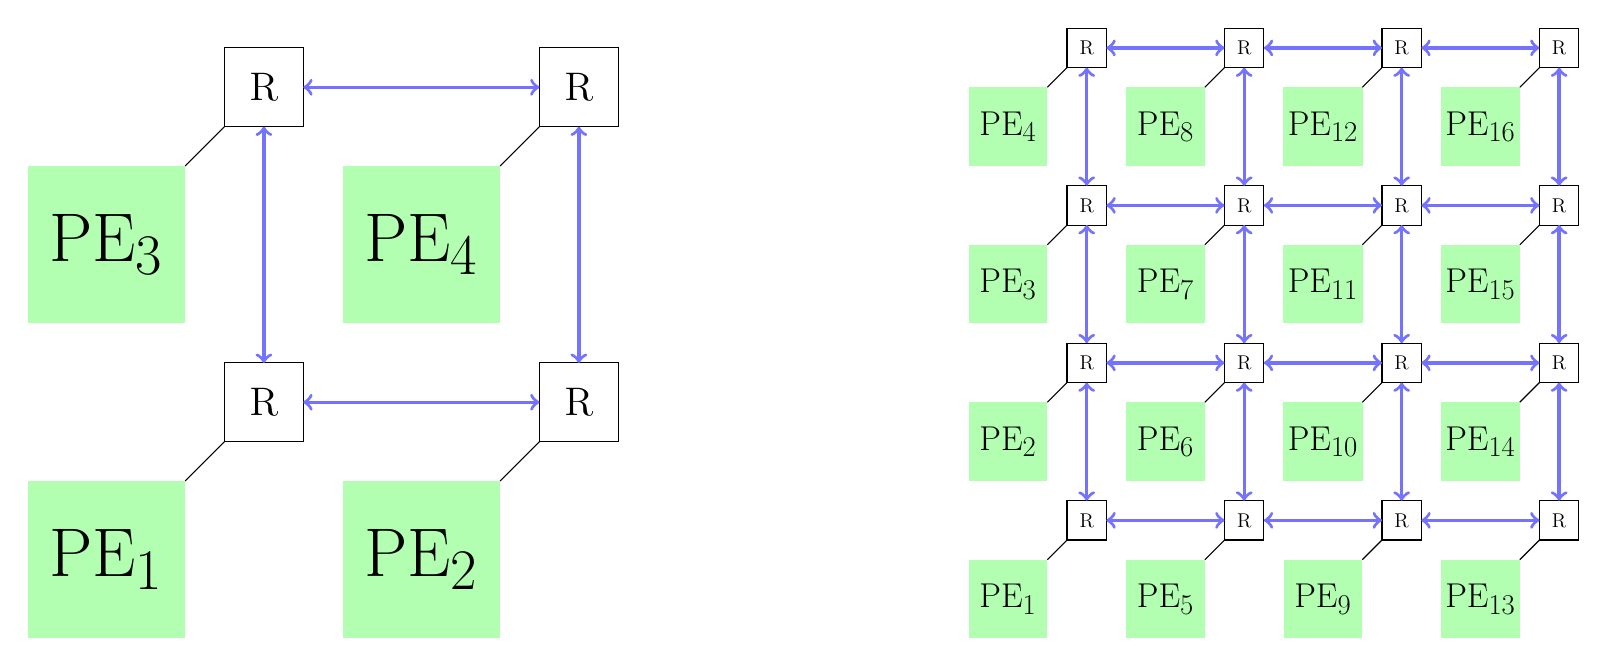
\begin{tikzpicture}
      
\begin{scope}[name prefix=orig-,xshift=-170]
  \node[rectangle,thick,minimum width = 2cm, minimum height=2cm,fill=green!30] (pe1) at (1,1) {\Huge PE$_1$};
  \node[rectangle,thick,minimum width = 2cm, minimum height=2cm,fill=green!30] (pe2) at (5,1) {\Huge PE$_2$};
  \node[rectangle,thick,minimum width = 2cm, minimum height=2cm,fill=green!30] (pe3) at (1,5) {\Huge PE$_3$};
  \node[rectangle,thick,minimum width = 2cm, minimum height=2cm,fill=green!30] (pe4) at (5,5) {\Huge PE$_4$};
  \foreach \x in {0,...,1}{
    \foreach \y in {0,...,1}{
       \pgfmathsetmacro{\xn}{\x*4}
       \pgfmathsetmacro{\yn}{\y*4} 
       \draw ({\xn + 2}, {\yn + 2}) -- ++(0.5,0.5);
       \draw ({\xn + 2.5},{\yn + 2.5}) rectangle ++(1,1) ++(-0.5,-0.5) node[font=\Large] {R};
      }
    }

  \foreach \x in {0,...,1}{
    \foreach \y in {0,...,1}{
      \pgfmathsetmacro{\xs}{\x*4+3}
      \pgfmathsetmacro{\ys}{\y*4+3}
      \pgfmathsetmacro{\xn}{\xs+3}
      \pgfmathsetmacro{\yn}{\ys+3}
      \pgfmathsetmacro{\xsm}{\x*4+3.5}
      \pgfmathsetmacro{\ysm}{\y*4+3.5}
      \pgfmathsetmacro{\xnm}{\xsm+3}
      \pgfmathsetmacro{\ynm}{\ysm+3}
      \ifnum\x<1
      \path[<->,very thick,blue!55] (\xsm,\ys) edge (\xnm,\ys);
      \fi
      \ifnum\y<1
      \path[<->,very thick,blue!55] (\xs,\ysm) edge (\xs,\ynm);
      \fi
      }
    }

\end{scope}



\begin{scope}[name prefix=transformed-,xshift=170,scale=0.5,,every node/.style={scale=0.5}]
  \node[rectangle,thick,minimum width = 2cm, minimum height=2cm,fill=green!30] (pe1) at (1,1) {\Huge PE$_1$};
  \node[rectangle,thick,minimum width = 2cm, minimum height=2cm,fill=green!30] (pe2) at (1,5) {\Huge PE$_2$};
  \node[rectangle,thick,minimum width = 2cm, minimum height=2cm,fill=green!30] (pe3) at (1,9) {\Huge PE$_3$};
  \node[rectangle,thick,minimum width = 2cm, minimum height=2cm,fill=green!30] (pe4) at (1,13) {\Huge PE$_4$};
  \node[rectangle,thick,minimum width = 2cm, minimum height=2cm,fill=green!30] (pe5) at (5,1) {\Huge PE$_5$};
  \node[rectangle,thick,minimum width = 2cm, minimum height=2cm,fill=green!30] (pe6) at (5,5) {\Huge PE$_6$};
  \node[rectangle,thick,minimum width = 2cm, minimum height=2cm,fill=green!30] (pe7) at (5,9) {\Huge PE$_7$};
  \node[rectangle,thick,minimum width = 2cm, minimum height=2cm,fill=green!30] (pe8) at (5,13) {\Huge PE$_8$};
  \node[rectangle,thick,minimum width = 2cm, minimum height=2cm,fill=green!30] (pe9) at (9,1) {\Huge PE$_9$};
  \node[rectangle,thick,minimum width = 2cm, minimum height=2cm,fill=green!30] (pe10) at (9,5) {\Huge PE$_{10}$};
  \node[rectangle,thick,minimum width = 2cm, minimum height=2cm,fill=green!30] (pe11) at (9,9) {\Huge PE$_{11}$};
  \node[rectangle,thick,minimum width = 2cm, minimum height=2cm,fill=green!30] (pe12) at (9,13) {\Huge PE$_{12}$};
  \node[rectangle,thick,minimum width = 2cm, minimum height=2cm,fill=green!30] (pe13) at (13,1) {\Huge PE$_{13}$};
  \node[rectangle,thick,minimum width = 2cm, minimum height=2cm,fill=green!30] (pe14) at (13,5) {\Huge PE$_{14}$};
  \node[rectangle,thick,minimum width = 2cm, minimum height=2cm,fill=green!30] (pe15) at (13,9) {\Huge PE$_{15}$};
  \node[rectangle,thick,minimum width = 2cm, minimum height=2cm,fill=green!30] (pe16) at (13,13) {\Huge PE$_{16}$};
  \foreach \x in {0,...,3}{
    \foreach \y in {0,...,3}{
       \pgfmathsetmacro{\xn}{\x*4}
       \pgfmathsetmacro{\yn}{\y*4} 
       \draw ({\xn + 2}, {\yn + 2}) -- ++(0.5,0.5);
       \draw ({\xn + 2.5},{\yn + 2.5}) rectangle ++(1,1) ++(-0.5,-0.5) node[font=\Large] {R};
      }
    }

  \foreach \x in {0,...,3}{
    \foreach \y in {0,...,3}{
      \pgfmathsetmacro{\xs}{\x*4+3}
      \pgfmathsetmacro{\ys}{\y*4+3}
      \pgfmathsetmacro{\xn}{\xs+3}
      \pgfmathsetmacro{\yn}{\ys+3}
      \pgfmathsetmacro{\xsm}{\x*4+3.5}
      \pgfmathsetmacro{\ysm}{\y*4+3.5}
      \pgfmathsetmacro{\xnm}{\xsm+3}
      \pgfmathsetmacro{\ynm}{\ysm+3}
      \ifnum\x<3
      \path[<->,very thick,blue!55] (\xsm,\ys) edge (\xnm,\ys);
      \fi
      \ifnum\y<3
      \path[<->,very thick,blue!55] (\xs,\ysm) edge (\xs,\ynm);
      \fi
      }
    }

\end{scope}
      \end{tikzpicture}
      }
	\caption{A comparison of the two different-sized meshes and the intuitive notion of their symmetries.}
	\label{fig:motivation_partial_symmetries}
\end{figure}

However, if we look at the group of automorphisms of the corresponding architecture graphs, we get a result that defies this intuition:
both architectures have the same groups of symmetries!
More precisely, their groups of automorphisms are isomorphic, they are dihedral groups on 4 points, $D_4$.
More concretely, there are only 8  possible structure-preserving transformations acting on these two topologies, which are the rotations of $90^\circ,180^\circ,270^\circ,360^\circ = 0^\circ$ and the reflections among each of the axes (horizontal, vertical and both diagonals).
We cannot, for example, divide the four-by-four mesh into a two-by-two mesh of two-by-two meshes, and rotate that larger two-by-two mesh by $90^\circ$ or one of the smaller ones by $90^\circ$.
These two operations both work locally, if we ignore the rest of the structure, but do not preserve the whole structure of the mesh, as illustrated by Figure~\ref{fig:partial_symmetries_4x4}.
The figure shows how a rotation on the bottom left $2 \times 2$ mesh breaks the communication structure.
Highlighted is the communication between $\PE_1$ and $\PE_3$, which changes from $2$ hops to $1$ hop in the transformation.

\begin{figure}[h]
	\centering
   \resizebox{0.95\textwidth}{!}{
      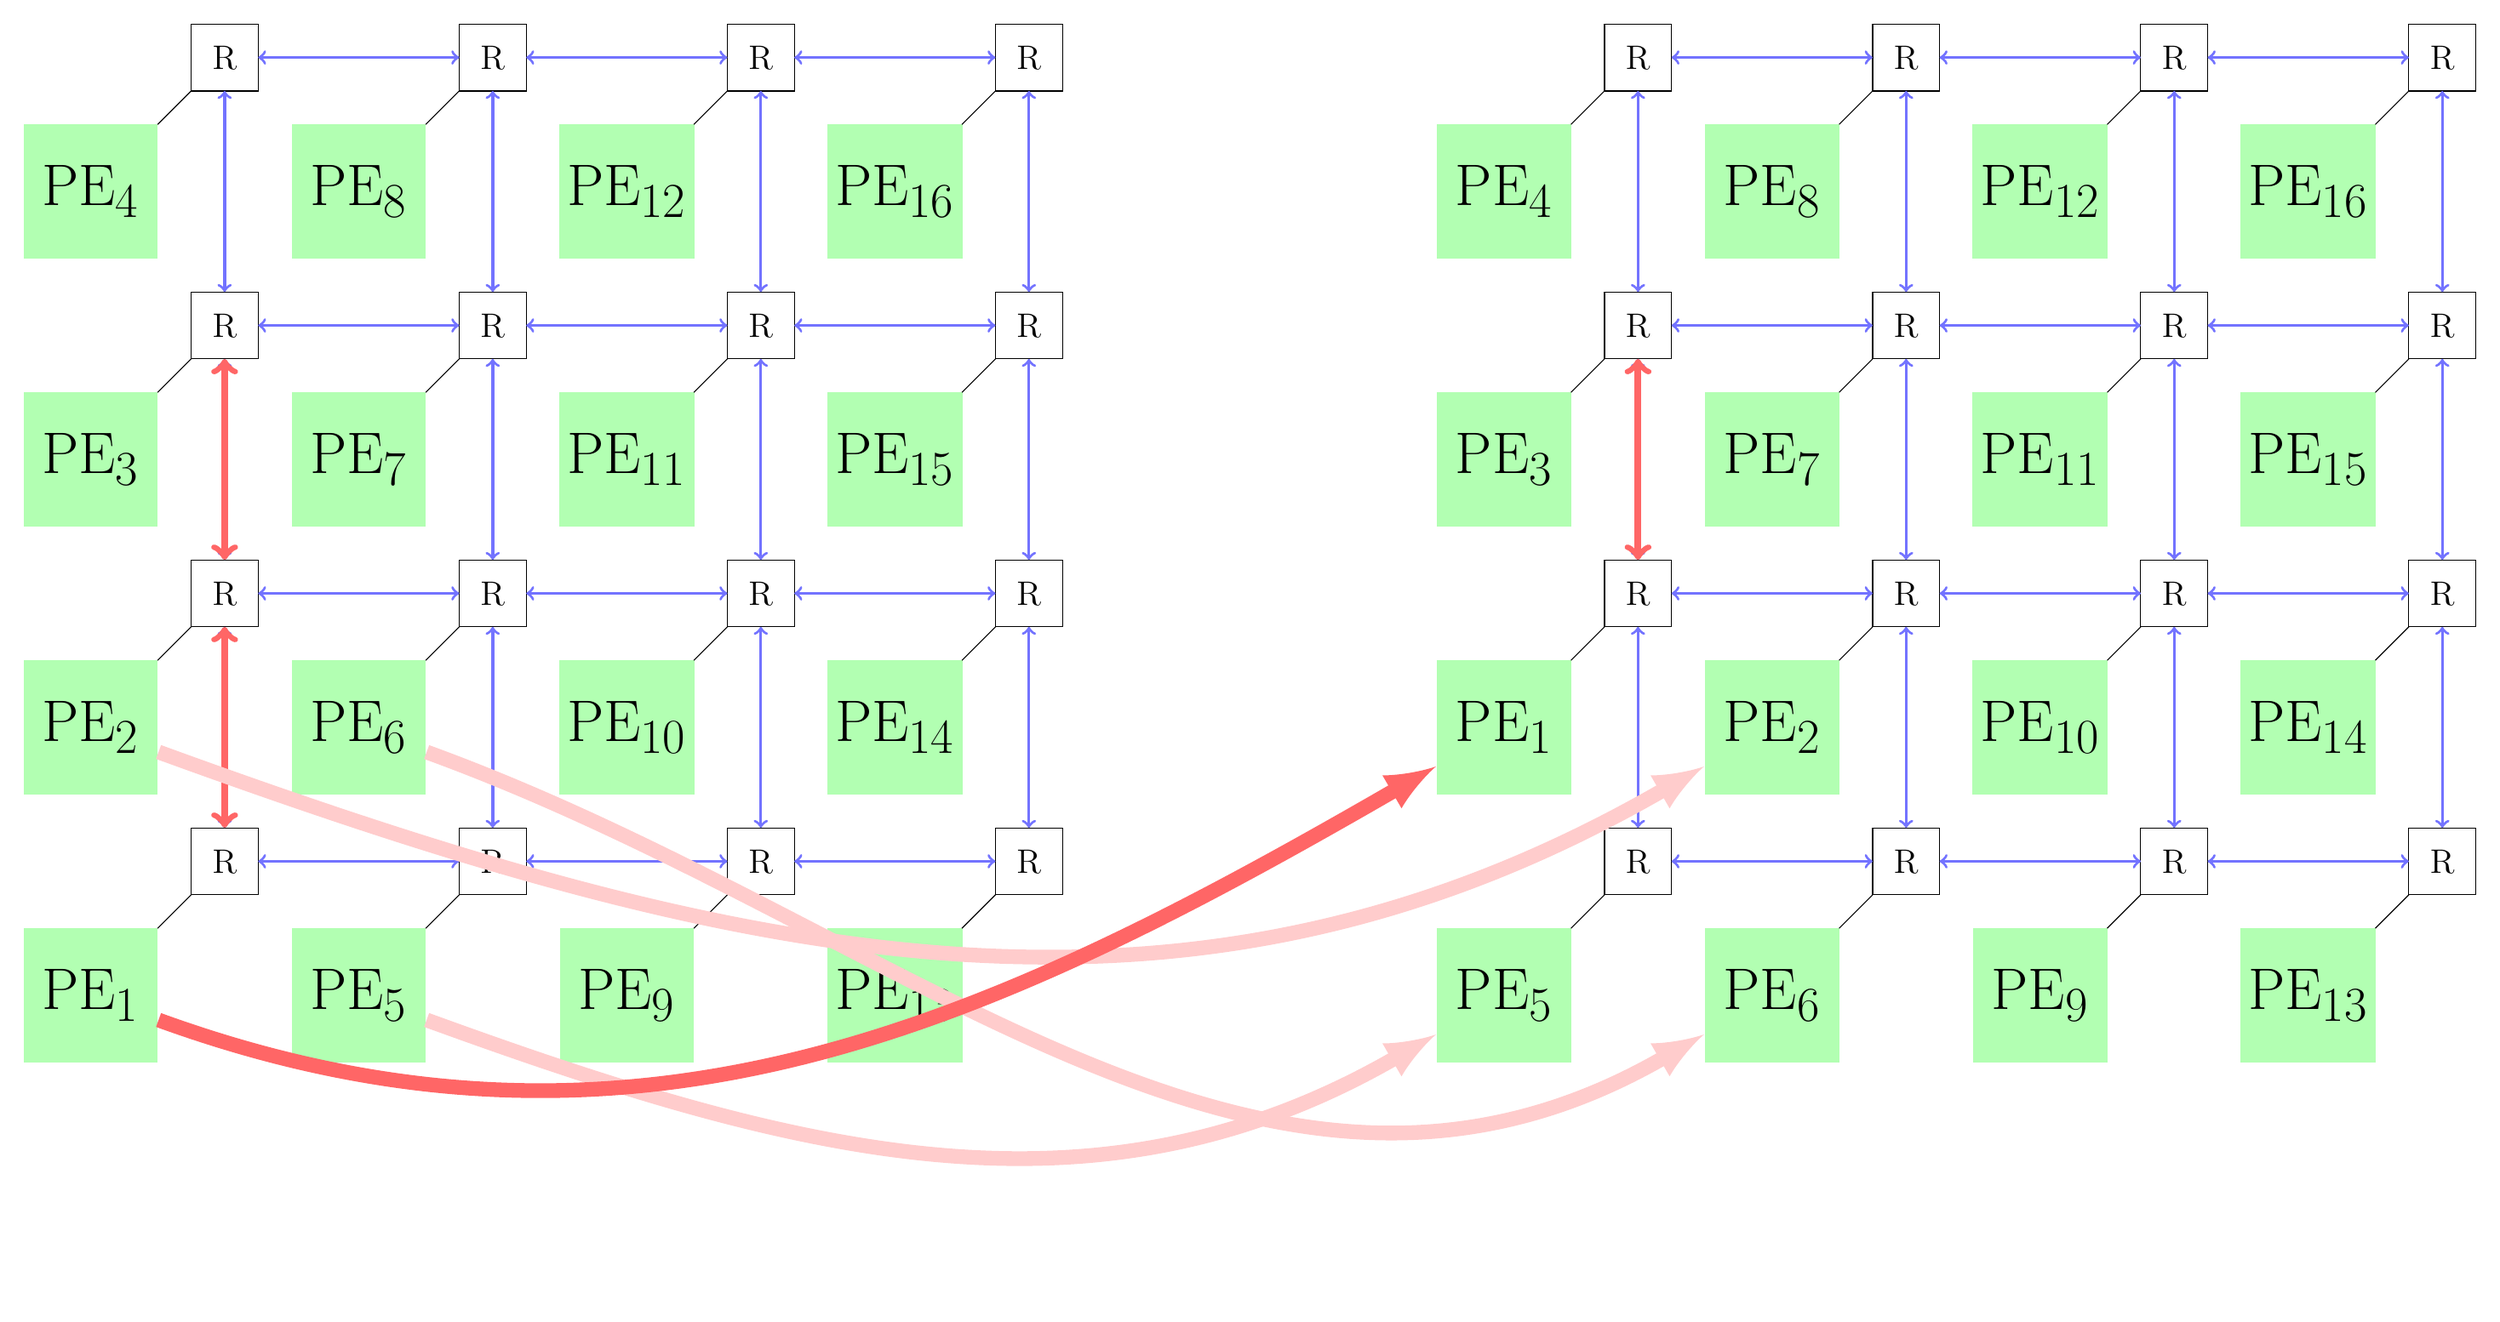
\begin{tikzpicture}
      \begin{scope}[name prefix=orig-]
  \node[rectangle,thick,minimum width = 2cm, minimum height=2cm,fill=green!30] (pe1) at (1,1) {\Huge PE$_1$};
  \node[rectangle,thick,minimum width = 2cm, minimum height=2cm,fill=green!30] (pe2) at (1,5) {\Huge PE$_2$};
  \node[rectangle,thick,minimum width = 2cm, minimum height=2cm,fill=green!30] (pe3) at (1,9) {\Huge PE$_3$};
  \node[rectangle,thick,minimum width = 2cm, minimum height=2cm,fill=green!30] (pe4) at (1,13) {\Huge PE$_4$};
  \node[rectangle,thick,minimum width = 2cm, minimum height=2cm,fill=green!30] (pe5) at (5,1) {\Huge PE$_5$};
  \node[rectangle,thick,minimum width = 2cm, minimum height=2cm,fill=green!30] (pe6) at (5,5) {\Huge PE$_6$};
  \node[rectangle,thick,minimum width = 2cm, minimum height=2cm,fill=green!30] (pe7) at (5,9) {\Huge PE$_7$};
  \node[rectangle,thick,minimum width = 2cm, minimum height=2cm,fill=green!30] (pe8) at (5,13) {\Huge PE$_8$};
  \node[rectangle,thick,minimum width = 2cm, minimum height=2cm,fill=green!30] (pe9) at (9,1) {\Huge PE$_9$};
  \node[rectangle,thick,minimum width = 2cm, minimum height=2cm,fill=green!30] (pe10) at (9,5) {\Huge PE$_{10}$};
  \node[rectangle,thick,minimum width = 2cm, minimum height=2cm,fill=green!30] (pe11) at (9,9) {\Huge PE$_{11}$};
  \node[rectangle,thick,minimum width = 2cm, minimum height=2cm,fill=green!30] (pe12) at (9,13) {\Huge PE$_{12}$};
  \node[rectangle,thick,minimum width = 2cm, minimum height=2cm,fill=green!30] (pe13) at (13,1) {\Huge PE$_{13}$};
  \node[rectangle,thick,minimum width = 2cm, minimum height=2cm,fill=green!30] (pe14) at (13,5) {\Huge PE$_{14}$};
  \node[rectangle,thick,minimum width = 2cm, minimum height=2cm,fill=green!30] (pe15) at (13,9) {\Huge PE$_{15}$};
  \node[rectangle,thick,minimum width = 2cm, minimum height=2cm,fill=green!30] (pe16) at (13,13) {\Huge PE$_{16}$};
  \foreach \x in {0,...,3}{
    \foreach \y in {0,...,3}{
       \pgfmathsetmacro{\xn}{\x*4}
       \pgfmathsetmacro{\yn}{\y*4} 
       \draw ({\xn + 2}, {\yn + 2}) -- ++(0.5,0.5);
       \draw ({\xn + 2.5},{\yn + 2.5}) rectangle ++(1,1) ++(-0.5,-0.5) node[font=\Large] {R};
      }
    }

  \foreach \x in {0,...,3}{
    \foreach \y in {0,...,3}{
      \pgfmathsetmacro{\xs}{\x*4+3}
      \pgfmathsetmacro{\ys}{\y*4+3}
      \pgfmathsetmacro{\xn}{\xs+3}
      \pgfmathsetmacro{\yn}{\ys+3}
      \pgfmathsetmacro{\xsm}{\x*4+3.5}
      \pgfmathsetmacro{\ysm}{\y*4+3.5}
      \pgfmathsetmacro{\xnm}{\xsm+3}
      \pgfmathsetmacro{\ynm}{\ysm+3}
      \ifnum\x<3
      \path[<->,very thick,blue!55] (\xsm,\ys) edge (\xnm,\ys);
      \fi
      \ifnum\y<3
      \path[<->,very thick,blue!55] (\xs,\ysm) edge (\xs,\ynm);
      \fi
      }
    }

      \path[<->,line width=1mm,red!60] (3,3.5) edge (3,6.5);
      \path[<->,line width=1mm,red!60] (3,7.5) edge (3,10.5);
\end{scope}

\begin{scope}[xshift=600,name prefix=transformed-]
  \node[rectangle,thick,minimum width = 2cm, minimum height=2cm,fill=green!30] (pe5) at (1,1) {\Huge PE$_5$};
  \node[rectangle,thick,minimum width = 2cm, minimum height=2cm,fill=green!30] (pe1) at (1,5) {\Huge PE$_1$};
  \node[rectangle,thick,minimum width = 2cm, minimum height=2cm,fill=green!30] (pe3) at (1,9) {\Huge PE$_3$};
  \node[rectangle,thick,minimum width = 2cm, minimum height=2cm,fill=green!30] (pe4) at (1,13) {\Huge PE$_4$};
  \node[rectangle,thick,minimum width = 2cm, minimum height=2cm,fill=green!30] (pe6) at (5,1) {\Huge PE$_6$};
  \node[rectangle,thick,minimum width = 2cm, minimum height=2cm,fill=green!30] (pe2) at (5,5) {\Huge PE$_2$};
  \node[rectangle,thick,minimum width = 2cm, minimum height=2cm,fill=green!30] (pe7) at (5,9) {\Huge PE$_7$};
  \node[rectangle,thick,minimum width = 2cm, minimum height=2cm,fill=green!30] (pe8) at (5,13) {\Huge PE$_8$};
  \node[rectangle,thick,minimum width = 2cm, minimum height=2cm,fill=green!30] (pe9) at (9,1) {\Huge PE$_9$};
  \node[rectangle,thick,minimum width = 2cm, minimum height=2cm,fill=green!30] (pe10) at (9,5) {\Huge PE$_{10}$};
  \node[rectangle,thick,minimum width = 2cm, minimum height=2cm,fill=green!30] (pe11) at (9,9) {\Huge PE$_{11}$};
  \node[rectangle,thick,minimum width = 2cm, minimum height=2cm,fill=green!30] (pe12) at (9,13) {\Huge PE$_{12}$};
  \node[rectangle,thick,minimum width = 2cm, minimum height=2cm,fill=green!30] (pe13) at (13,1) {\Huge PE$_{13}$};
  \node[rectangle,thick,minimum width = 2cm, minimum height=2cm,fill=green!30] (pe14) at (13,5) {\Huge PE$_{14}$};
  \node[rectangle,thick,minimum width = 2cm, minimum height=2cm,fill=green!30] (pe15) at (13,9) {\Huge PE$_{15}$};
  \node[rectangle,thick,minimum width = 2cm, minimum height=2cm,fill=green!30] (pe16) at (13,13) {\Huge PE$_{16}$};
  \foreach \x in {0,...,3}{
    \foreach \y in {0,...,3}{
       \pgfmathsetmacro{\xn}{\x*4}
       \pgfmathsetmacro{\yn}{\y*4} 
       \draw ({\xn + 2}, {\yn + 2}) -- ++(0.5,0.5);
       \draw ({\xn + 2.5},{\yn + 2.5}) rectangle ++(1,1) ++(-0.5,-0.5) node[font=\Large] {R};
      }
    }

  \foreach \x in {0,...,3}{
    \foreach \y in {0,...,3}{
      \pgfmathsetmacro{\xs}{\x*4+3}
      \pgfmathsetmacro{\ys}{\y*4+3}
      \pgfmathsetmacro{\xn}{\xs+3}
      \pgfmathsetmacro{\yn}{\ys+3}
      \pgfmathsetmacro{\xsm}{\x*4+3.5}
      \pgfmathsetmacro{\ysm}{\y*4+3.5}
      \pgfmathsetmacro{\xnm}{\xsm+3}
      \pgfmathsetmacro{\ynm}{\ysm+3}
      \ifnum\x<3
      \path[<->,very thick,blue!55] (\xsm,\ys) edge (\xnm,\ys);
      \fi
      \ifnum\y<3
      \path[<->,very thick,blue!55] (\xs,\ysm) edge (\xs,\ynm);
      \fi
      }
    }

      \path[<->,line width=1mm,red!60] (3,7.5) edge (3,10.5);
\end{scope}

\draw (orig-pe2) edge[-{latex},line width=2.2mm, color=red!20,in=210,out=340,looseness=1]  (transformed-pe2);
\draw (orig-pe5) edge[-{latex},line width=2.2mm, color=red!20,in=210,out=340,looseness=1]  (transformed-pe5);
\draw (orig-pe6) edge[-{latex},line width=2.2mm, color=red!20,in=210,out=340,looseness=1]  (transformed-pe6);
\draw (orig-pe1) edge[-{latex},line width=2.2mm, color=red!60,in=210,out=340,looseness=1]  (transformed-pe1);
      \end{tikzpicture}
      }
	\caption{An example of a local symmetry that is not a global symmetry of a $4 \times 4$ mesh.}
	\label{fig:partial_symmetries_4x4}
\end{figure}

For the mathematical formalization of this intuitive notion of local symmetries, in this section, we follow~\cite{lawson_inverse_semigroups}.
There are essentially two equivalent ways of formalizing this intuitive notion of local symmetries, inverse semigroups and ordered groupoids.
We will consider the formalization using inverse semigroups, as it is conceptually simpler for computations, and mathematically equally as powerful.
In the case of global symmetries, there are concrete transformations of architectures and mappings, which correspond to abstract groups.
For partial symmetries, we will consider partial transformations of mappings, which we will model as partial permutations, and these partial permutations (transformations) have a corresponding abstract inverse semigroup.

We start by defining partial functions and partial permutations.
\begin{defn}
Let X,Y be sets.
A \emph{partial function} $f: X \rightarrow Y$ is a function from a subset of $X$ to a subset of $Y$.
We denote the domain of $f$ by $\dom(f)$ the codomain of $f$ by $\cod(f)$.
Thus, the partial function $f: X \rightarrow Y$ is a (total) function $f: \dom(f) \rightarrow \cod(f)$
\end{defn}

\begin{defn}
Let $X$ be a set.
A partial function $f: X \rightarrow X$ from $X$ to itself is called a \emph{partial permutation} if the (total) function $f: \dom(f) \rightarrow \cod(f)$ is a bijection between $\dom(f)$ and $\cod(f)$.
\end{defn}

\begin{figure}[h]
	\centering
   \resizebox{0.95\textwidth}{!}{
      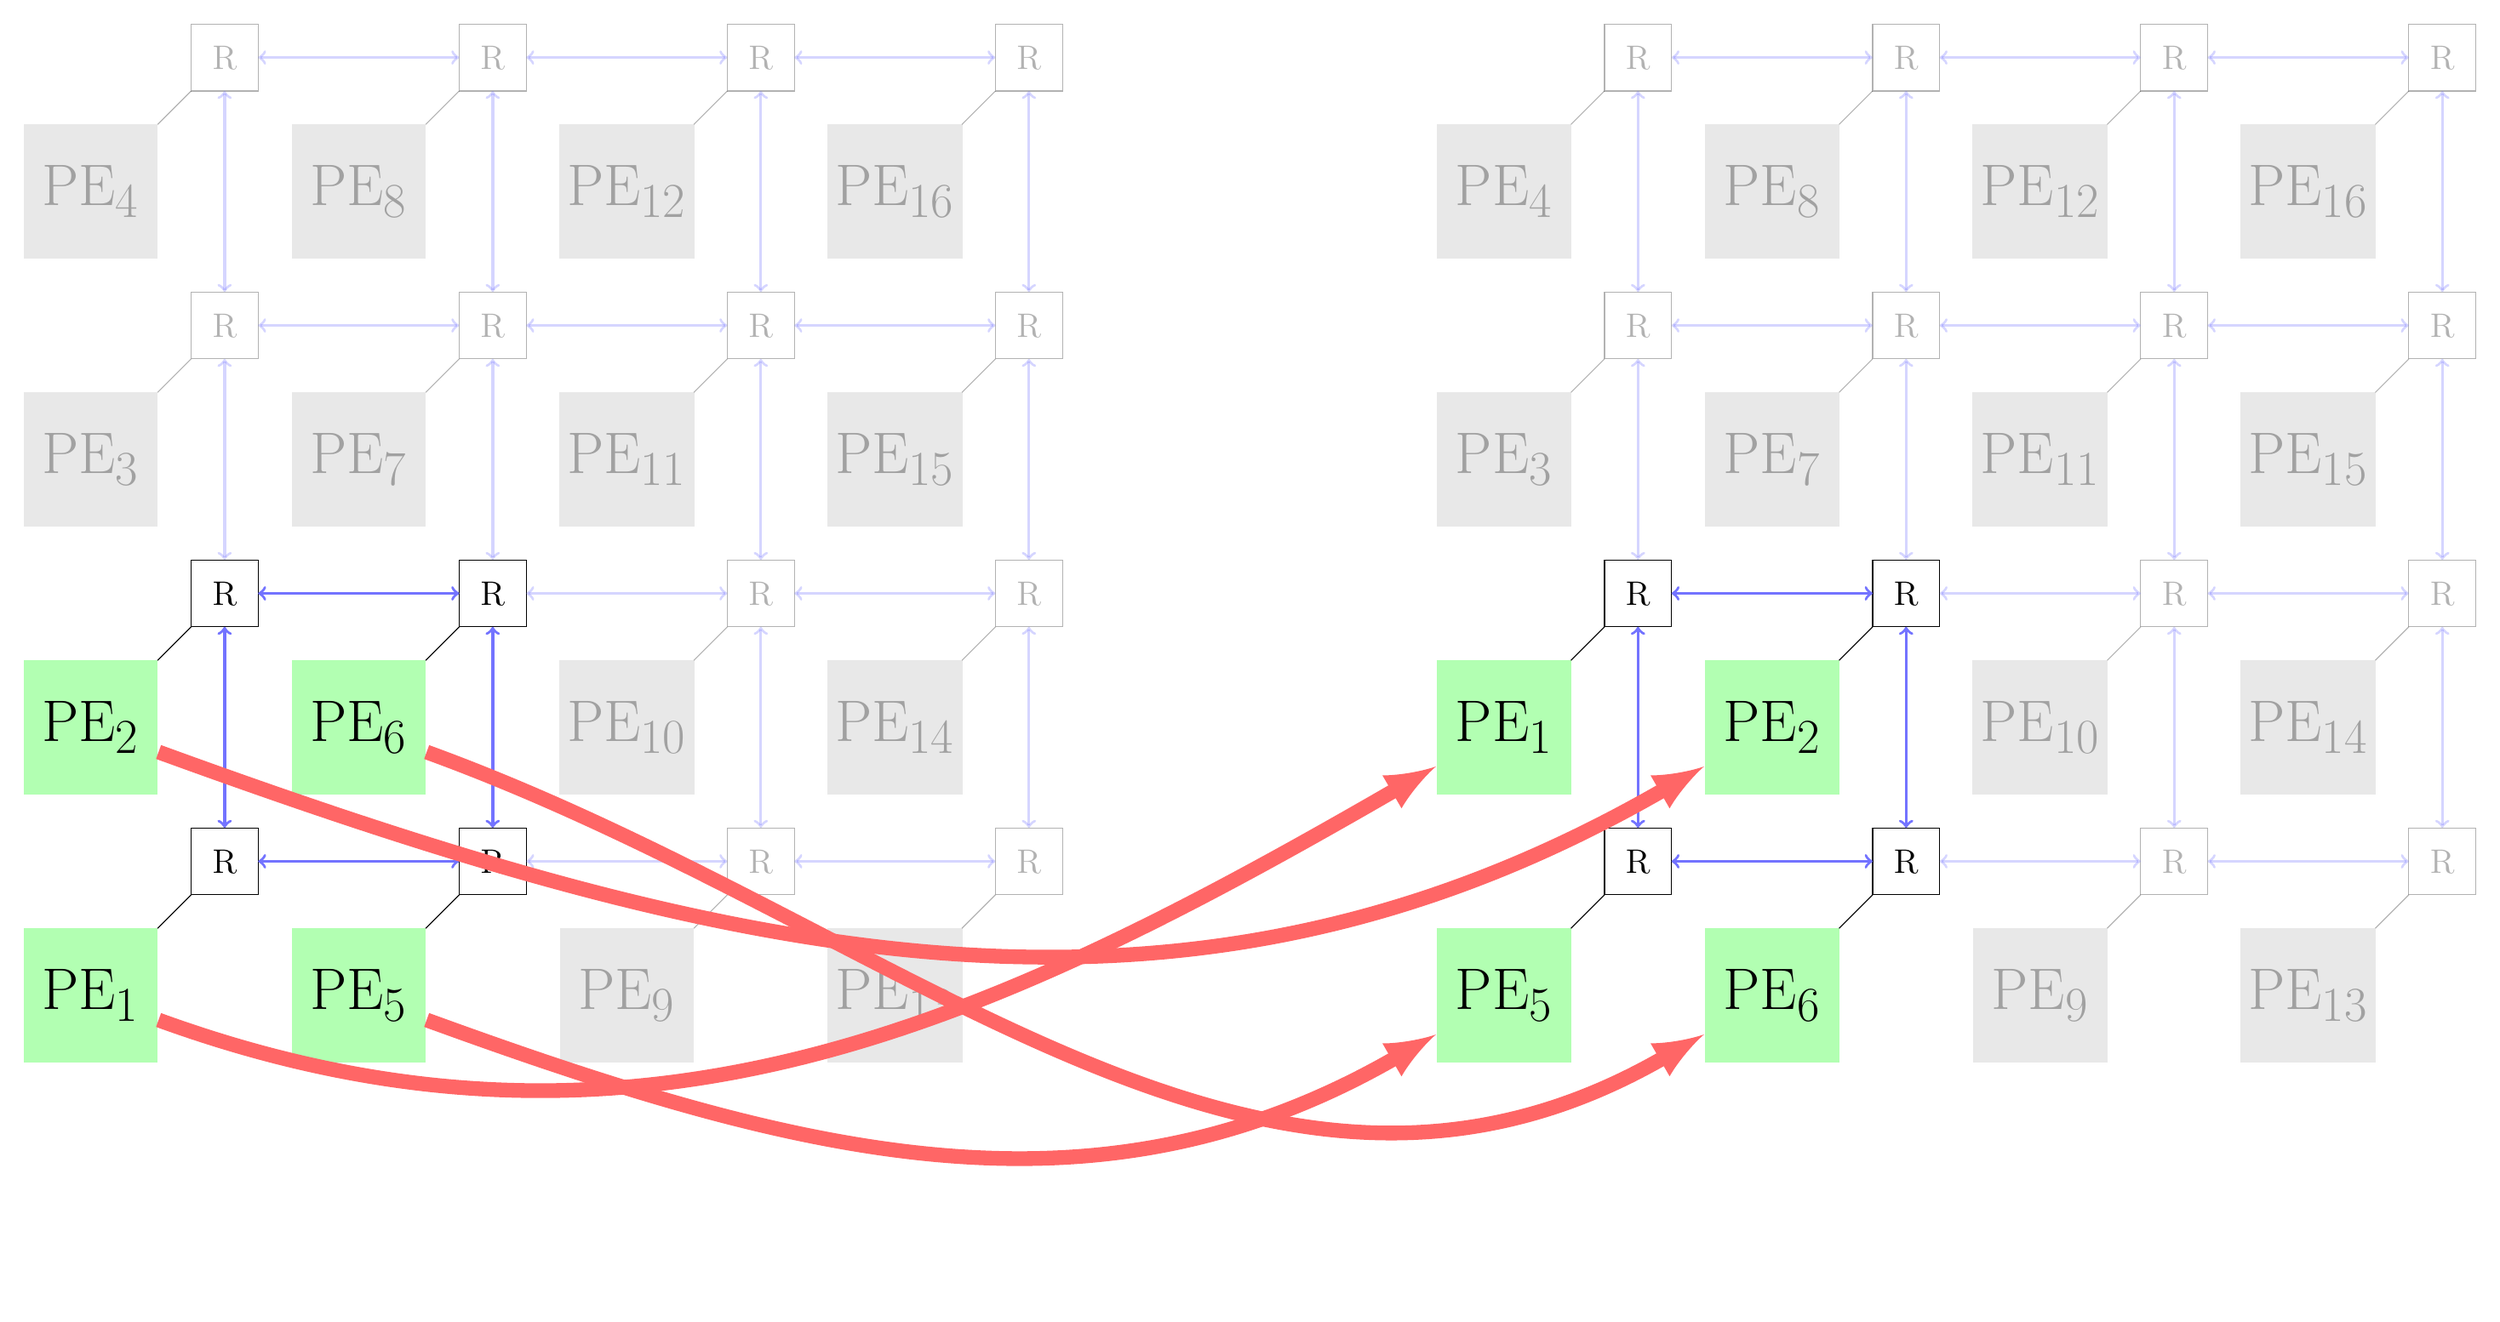
\begin{tikzpicture}
      \begin{scope}[name prefix=orig-]
  \node[rectangle,thick,minimum width = 2cm, minimum height=2cm,fill=green!30] (pe1) at (1,1) {\Huge PE$_1$};
  \node[rectangle,thick,minimum width = 2cm, minimum height=2cm,fill=green!30] (pe2) at (1,5) {\Huge PE$_2$};
  \node[rectangle,thick,minimum width = 2cm, minimum height=2cm,fill=gray!60,opacity=0.3] (pe3) at (1,9) {\Huge PE$_3$};
  \node[rectangle,thick,minimum width = 2cm, minimum height=2cm,fill=gray!60,opacity=0.3] (pe4) at (1,13) {\Huge PE$_4$};
  \node[rectangle,thick,minimum width = 2cm, minimum height=2cm,fill=green!30] (pe5) at (5,1) {\Huge PE$_5$};
  \node[rectangle,thick,minimum width = 2cm, minimum height=2cm,fill=green!30] (pe6) at (5,5) {\Huge PE$_6$};
  \node[rectangle,thick,minimum width = 2cm, minimum height=2cm,fill=gray!60,opacity=0.3] (pe7) at (5,9) {\Huge PE$_7$};
  \node[rectangle,thick,minimum width = 2cm, minimum height=2cm,fill=gray!60,opacity=0.3] (pe8) at (5,13) {\Huge PE$_8$};
  \node[rectangle,thick,minimum width = 2cm, minimum height=2cm,fill=gray!60,opacity=0.3] (pe9) at (9,1) {\Huge PE$_9$};
  \node[rectangle,thick,minimum width = 2cm, minimum height=2cm,fill=gray!60,opacity=0.3] (pe10) at (9,5) {\Huge PE$_{10}$};
  \node[rectangle,thick,minimum width = 2cm, minimum height=2cm,fill=gray!60,opacity=0.3] (pe11) at (9,9) {\Huge PE$_{11}$};
  \node[rectangle,thick,minimum width = 2cm, minimum height=2cm,fill=gray!60,opacity=0.3] (pe12) at (9,13) {\Huge PE$_{12}$};
  \node[rectangle,thick,minimum width = 2cm, minimum height=2cm,fill=gray!60,opacity=0.3] (pe13) at (13,1) {\Huge PE$_{13}$};
  \node[rectangle,thick,minimum width = 2cm, minimum height=2cm,fill=gray!60,opacity=0.3] (pe14) at (13,5) {\Huge PE$_{14}$};
  \node[rectangle,thick,minimum width = 2cm, minimum height=2cm,fill=gray!60,opacity=0.3] (pe15) at (13,9) {\Huge PE$_{15}$};
  \node[rectangle,thick,minimum width = 2cm, minimum height=2cm,fill=gray!60,opacity=0.3] (pe16) at (13,13) {\Huge PE$_{16}$};
  \foreach \x in {0,...,3}{
    \foreach \y in {0,...,3}{
       \pgfmathsetmacro{\xn}{\x*4}
       \pgfmathsetmacro{\yn}{\y*4} 
       \draw[opacity=0.3] ({\xn + 2}, {\yn + 2}) -- ++(0.5,0.5);
       \draw[opacity=0.3] ({\xn + 2.5},{\yn + 2.5}) rectangle ++(1,1) ++(-0.5,-0.5) node[font=\Large,opacity=0.3] {R};
      \ifnum\x<2
      \ifnum\y<2
       \draw ({\xn + 2}, {\yn + 2}) -- ++(0.5,0.5);
       \draw ({\xn + 2.5},{\yn + 2.5}) rectangle ++(1,1) ++(-0.5,-0.5) node[font=\Large] {R};
       \fi
       \fi

      }
    }

  \foreach \x in {0,...,3}{
    \foreach \y in {0,...,3}{
      \pgfmathsetmacro{\xs}{\x*4+3}
      \pgfmathsetmacro{\ys}{\y*4+3}
      \pgfmathsetmacro{\xn}{\xs+3}
      \pgfmathsetmacro{\yn}{\ys+3}
      \pgfmathsetmacro{\xsm}{\x*4+3.5}
      \pgfmathsetmacro{\ysm}{\y*4+3.5}
      \pgfmathsetmacro{\xnm}{\xsm+3}
      \pgfmathsetmacro{\ynm}{\ysm+3}

      \ifnum\x<3
      \path[<->,very thick,blue!55,opacity=0.3] (\xsm,\ys) edge (\xnm,\ys);
      \fi
      \ifnum\y<3
      \path[<->,very thick,blue!55,opacity=0.3] (\xs,\ysm) edge (\xs,\ynm);
      \fi

      \ifnum\x<1
      \ifnum\y<2
      \path[<->,very thick,blue!55] (\xsm,\ys) edge (\xnm,\ys);
       \fi
       \fi
      \ifnum\y<1
      \ifnum\x<2
      \path[<->,very thick,blue!55] (\xs,\ysm) edge (\xs,\ynm);
       \fi
       \fi
      
      }
    }

\end{scope}

\begin{scope}[xshift=600,name prefix=transformed-]
  \node[rectangle,thick,minimum width = 2cm, minimum height=2cm,fill=green!30] (pe5) at (1,1) {\Huge PE$_5$};
  \node[rectangle,thick,minimum width = 2cm, minimum height=2cm,fill=green!30] (pe1) at (1,5) {\Huge PE$_1$};
  \node[rectangle,thick,minimum width = 2cm, minimum height=2cm,fill=gray!60,opacity=0.3] (pe3) at (1,9) {\Huge PE$_3$};
  \node[rectangle,thick,minimum width = 2cm, minimum height=2cm,fill=gray!60,opacity=0.3] (pe4) at (1,13) {\Huge PE$_4$};
  \node[rectangle,thick,minimum width = 2cm, minimum height=2cm,fill=green!30] (pe6) at (5,1) {\Huge PE$_6$};
  \node[rectangle,thick,minimum width = 2cm, minimum height=2cm,fill=green!30] (pe2) at (5,5) {\Huge PE$_2$};
  \node[rectangle,thick,minimum width = 2cm, minimum height=2cm,fill=gray!60,opacity=0.3] (pe7) at (5,9) {\Huge PE$_7$};
  \node[rectangle,thick,minimum width = 2cm, minimum height=2cm,fill=gray!60,opacity=0.3] (pe8) at (5,13) {\Huge PE$_8$};
  \node[rectangle,thick,minimum width = 2cm, minimum height=2cm,fill=gray!60,opacity=0.3] (pe9) at (9,1) {\Huge PE$_9$};
  \node[rectangle,thick,minimum width = 2cm, minimum height=2cm,fill=gray!60,opacity=0.3] (pe10) at (9,5) {\Huge PE$_{10}$};
  \node[rectangle,thick,minimum width = 2cm, minimum height=2cm,fill=gray!60,opacity=0.3] (pe11) at (9,9) {\Huge PE$_{11}$};
  \node[rectangle,thick,minimum width = 2cm, minimum height=2cm,fill=gray!60,opacity=0.3] (pe12) at (9,13) {\Huge PE$_{12}$};
  \node[rectangle,thick,minimum width = 2cm, minimum height=2cm,fill=gray!60,opacity=0.3] (pe13) at (13,1) {\Huge PE$_{13}$};
  \node[rectangle,thick,minimum width = 2cm, minimum height=2cm,fill=gray!60,opacity=0.3] (pe14) at (13,5) {\Huge PE$_{14}$};
  \node[rectangle,thick,minimum width = 2cm, minimum height=2cm,fill=gray!60,opacity=0.3] (pe15) at (13,9) {\Huge PE$_{15}$};
  \node[rectangle,thick,minimum width = 2cm, minimum height=2cm,fill=gray!60,opacity=0.3] (pe16) at (13,13) {\Huge PE$_{16}$};
  \foreach \x in {0,...,3}{
    \foreach \y in {0,...,3}{
       \pgfmathsetmacro{\xn}{\x*4}
       \pgfmathsetmacro{\yn}{\y*4} 
       \draw[opacity=0.3] ({\xn + 2}, {\yn + 2}) -- ++(0.5,0.5);
       \draw[opacity=0.3] ({\xn + 2.5},{\yn + 2.5}) rectangle ++(1,1) ++(-0.5,-0.5) node[font=\Large,opacity=0.3] {R};
      \ifnum\x<2
      \ifnum\y<2
       \draw ({\xn + 2}, {\yn + 2}) -- ++(0.5,0.5);
       \draw ({\xn + 2.5},{\yn + 2.5}) rectangle ++(1,1) ++(-0.5,-0.5) node[font=\Large] {R};
       \fi
       \fi
      }
    }

  \foreach \x in {0,...,3}{
    \foreach \y in {0,...,3}{
      \pgfmathsetmacro{\xs}{\x*4+3}
      \pgfmathsetmacro{\ys}{\y*4+3}
      \pgfmathsetmacro{\xn}{\xs+3}
      \pgfmathsetmacro{\yn}{\ys+3}
      \pgfmathsetmacro{\xsm}{\x*4+3.5}
      \pgfmathsetmacro{\ysm}{\y*4+3.5}
      \pgfmathsetmacro{\xnm}{\xsm+3}
      \pgfmathsetmacro{\ynm}{\ysm+3}

      \ifnum\x<3
      \path[<->,very thick,blue!55,opacity=0.3] (\xsm,\ys) edge (\xnm,\ys);
      \fi
      \ifnum\y<3
      \path[<->,very thick,blue!55,opacity=0.3] (\xs,\ysm) edge (\xs,\ynm);
      \fi

      \ifnum\x<1
      \ifnum\y<2
      \path[<->,very thick,blue!55] (\xsm,\ys) edge (\xnm,\ys);
       \fi
       \fi
      \ifnum\y<1
      \ifnum\x<2
      \path[<->,very thick,blue!55] (\xs,\ysm) edge (\xs,\ynm);
       \fi
       \fi
      
      }
    }

\end{scope}

\draw (orig-pe2) edge[-{latex},line width=2.2mm, color=red!60,in=210,out=340,looseness=1]  (transformed-pe2);
\draw (orig-pe5) edge[-{latex},line width=2.2mm, color=red!60,in=210,out=340,looseness=1]  (transformed-pe5);
\draw (orig-pe6) edge[-{latex},line width=2.2mm, color=red!60,in=210,out=340,looseness=1]  (transformed-pe6);
\draw (orig-pe1) edge[-{latex},line width=2.2mm, color=red!60,in=210,out=340,looseness=1]  (transformed-pe1);
      \end{tikzpicture}
      }
	\caption{The transformation of Figure~\ref{fig:partial_symmetries_4x4} as a partial permutation.}
	\label{fig:example_partial_permutation}
\end{figure}

We can think of partial functions thus as functions that are not defined everywhere, and partial permutations, accordingly, are not defined everywhere.
For example, the partial permutation $f : \{1,\ldots,16\} \rightarrow \{1,\ldots,16\}$ defined as $f(1) = 2, f(2) = 6, f(5) = 1, f(6) = 5$ is a rotation of the bottom-left $2 \times 2$-mesh in the $4\times 4$-mesh depicted in Figure~\ref{fig:partial_symmetries_4x4}, but is not defined on the rest of the architcture.
This is a partial symmetry of the $4\times 4$-mesh.
This partial permutation is depicted in Figure~\ref{fig:example_partial_permutation}.
We can write it also as:
\begin{equation*}
\left(
\begin{array}{llllllllllllllll}
 1 & 2 & 3 & 4 & 5 & 6 & 7 & 8 & 9 & 10 & 11 & 12 & 13 & 14 & 15 & 16 \\
 2 & 6 & - & - & 1 & 5 & - & - & - &  - &  - &  - &  - &  - &  - & -
\end{array}
\right)
\end{equation*}
Because the set $\{1,\ldots,16\}$ is understood from context, we can also write it, shorter, as:
\begin{equation*}
\left(
\begin{array}{llll}
1 & 2 & 5 & 6 \\
2 & 6 &  1 & 5
\end{array}
\right)
\end{equation*}

We also use a notation similar to the cycle notation of group theory, where we use a cicle with round brackets to denote a full cycle, where the last element maps to the first.
Square brackets to denote when this is not the case, i.e. the function is not defined on the last element of that cycle. In this notation, singleton cycles cannot be omitted as in the case of groups.
In other words, fixed points have to be represented as one-element cycles.
The partial permutation from Figure~\ref{fig:example_partial_permutation} can thus be written much more compactly as: $(1,2,6,5)$.
This is a full cycle, but it is only defined on the subset $\{1,2,5,6\}$.
In the group context, the cycle $(1,2,6,5)$ as an element of the symmetric group on 16 points, would instead mean the (complete) permutation that fixes $\{3,4,7,8,9,10,11,12,13,14,15,16\}$.
As a partial permutation in cycle notation we would write this as:
 \[(1,2,6,5)(3)(4)(7)(8)(9)(10)(11)(12)(13)(14)(15)(16) \]
A different example of a partial permutation is the partial permutation that moves the first column to the right (and is not defined on the rest), as a cycle: $[1,5][2,6][3,7][4,8]$.
On the other hand, the partial permutation that is a diagonal reflection on the bottom-left $2 \times 2$ (sub)mesh is, in cycle notation, $(2,5)(1)(6)$.
These two partial permutations can also be written in the matrix notation from above as:

\begin{equation*}
\left(
\begin{array}{llll}
1 & 2 & 3 & 4 \\
5 & 6 & 7 & 8 
\end{array}
\right)
\quad
\left(
\begin{array}{llll}
1 & 2 & 5 & 6 \\
1 & 5 & 2 & 6
\end{array}
\right)
\end{equation*}

For computations~\cite{east2019semigroups}, the three notations can be interpreted to make different data structures that make different opperations more efficient, like application of the partial function (as an array look-up), for sparse partial permutations (as lookups in key-value pairs), or cycles for efficient multiplication (as concatenation). They have different benefits and drawbacks. For readability though, the cycle notation is the most compact one, and the one we will use for the rest of this thesis.

Just as for groups, we can define the (left) action of a semigroup:
\begin{defn}
Let $S$ be a semigroup and $X$ be a set. We say that $S$ \emph{acts} on $X$ (on the left) if there is a function $\cdot : S \times X \rightarrow X$ such that $(ab) \cdot x = a \cdot (b \cdot x)$. If $S$ is a monoid with identity $1$ and the function $\cdot$ satisfies the condition $1 \cdot x = x$ for all $x \in X$, we say that the action is a monoid action.
\end{defn}

The action of a semigroup of partial permutations on an architecture works the same as with groups, except it does not work on the whole architecture.
Let $f$ be a partial permutation on an architecture $A$, and $m : K \rightarrow A$ be a mapping on that architecture.
If the partial permutation is defined on all cores that $m$ maps to, i.e., $\im(m) \subseteq \dom(f)$, then we can use the action of the semigroup of partial permutations of $A$ to define another mapping $fm$ by $fm(t) = f \cdot m(t)$ for all $t$ in $K$.
If $f$ is not defined on some of the cores of $m$, i.e., $\im(m) \not \subseteq \dom(f)$, then we cannot define $fm$. In this way, $f$ also defines a partial permutation $\hat f$ on the set of mappings $M \subseteq \{ m : K \rightarrow A \} =: A^K$.

Consider for example the mapping of an application with three tasks to the $4 \times 4$-mesh defined by $m_1(t_1) = m_1(t_3) = \PE_1$ and $m_1(t_2) = \PE_5$, which we can also write as the vector $m_1 = (1,5,1)$.
Then the partial permutation $(1,2,6,5)$ from Figure~\ref{fig:example_partial_permutation} above defines the mapping $(1,2,6,5)m_1 = (2,1,2)$.
Similarly, the action of the partial permutation $(2,5)(1)(6)$ yields a new mapping, $(2,5)(1)(6)m_1 = (1,2,1)$.
However, since the translation $\tau = [1,5][2,6][3,7][4,8]$ is not defined on $\PE_5 = m_1(t_2)$, we cannot define $[1,5][2,6][3,7][4,8]$ as a mapping.
Formally we can say that the partial permutations $\widehat{(1,2,6,5)}$ and $\widehat{(2,5)(1)(6)}$ are defined on $m_1$, but $\widehat{[1,5][2,6][3,7][4,8]}$ is not defined on $m_1$.

What happens with application symmetries? As defined here, the edges of the application $K$ are the (data) dependencies of a computation process (or task).
All dependencies have to be respected, which means that considering partial symmetries of the application can lead to non-determinstic or faulty behavior. 

We are now ready to formally define the set of partial symmetries of architectures and mappings, as in the case of groups.
Recall that a mapping $m: K \rightarrow A$ can be seen as a morphism of graphs from $M$ to $A$.
In particular, every mapping $m$ defines a subgraph $m(K) \leq A$.
This subgraph has a node $m(t) \in V_A$ for every \ac{PE} in the architecture $A$ that is used in a mapping, and similarly an edge $(m(t_1),m(t_2)) \in E_A$ for every communication primitive where a channel is mapped to.
Precisely the isomorphism of these subgraphs is what defines the partial symmetries of the architecture. 

\begin{defn}[$\AutSemi$]
   Let $A$ be an architecture graph.
   The set of partial symmetries of the architecture graph $\AutSemi(A)$ is the set of partial labed-graph isomorphisms of $A$, i.e. the partial permutations $\varphi$ of $V_A$ which induce an isomorphism of labeled graphs between $\dom(\varphi)$ and $\cod(\varphi)$.
\index{$\AutSemi$}
\end{defn}

As motivated above, $\AutSemi(A)$ acts on the set of mappings $M$, just as $\operatorname{Aut}(A)$ the group of (total) symmetries does.
This action induces (and the action of the group $\operatorname{Aut}(K)$) define together an embedding on $\AutSemi(M) \leq \mathcal{I}(M)$, the inverse semigroup of partial permutations on $M$, which is how we define $\AutSemi(M)$.

In inverse semigroups, not every element has an inverse, only a pseudo-inverse. 
Consider the identity partial permutation on the lower-left $2\times 2$-\ac{NoC} in the $4 \times 4$ mesh, $i = (1)(2)(5)(6)$.
This identity partial permutation is an \emph{idempotent}\index{idempotent}, which means that $i^2 = i$, which implies that $i^{-1} = i$.
Groups, in contrast, have precisely one idempotent, the identity element.
The set of idempotents of a semigroup plays an important role in describing the structure of the semigroup~\cite{lawson_inverse_semigroups}.
If we then consider the translation $\tau$ from above, we can multiply $\tau i = [1,5][2,6]$, which is defined only on two cores.
If we muliply it with the pseudoinverse of $i$, $i^{-1} = i$, we get $\tau i i^{-1} = \tau i i = \tau i \neq \tau$.
There is no way we can get $\tau$ back from $\tau i$, since $\tau$ is defined on $4$ cores.

Just as with groups, we can define orbits for inverse semigroups.
However, due to the one-way nature of some multiplication operation, the orbit of a semigroup is more complicated.
Let $X$ be a set and let $S$ be a semigroup acting on $X$.
Then, for an element $x \in X$, we can think of the \emph{orbit graph} of $x$ as a directed graph $\mathbb{O} = (V,E)$ where $V = \{ s x \mid s \in S \}$.
The edges $E$ are defined by the action, namely an edge $e = (v,w)$ is added for every $v,w$ for which there exists an $s \in S$ such that $v = s w$.
This directed graph is clearly connected, but not strongly connected.
The \acp{s.c.c.} of this orbit graph\index{\ac{s.c.c.}} define equivalence classes and play the role that orbits played in group actions for our application to software synthesis.

By definition of $\AutSemi(A)$, for a partial symmetry $f \in \AutSemi(A)$ and a mapping $m$ we know that if the mapping $fm$ is defined, then the two subgraphs $fm(K) \cong m(K) \leq A$ are isomorphic.
We also get an isomorphism between the two subgraphs by Lemma~\ref{lem:symmetry_to_iso}
\begin{lem}
\label{lem:symmetry_to_iso}
Let $m : T \rightarrow A$ be a mapping and let $f \in \AutSemi(A)$ be a partial automorphism of the architecture such that $\im(m) \subseteq \dom(f)$.
Then, the two graphs $m(K)$ and $(fm)(K)$ are isomorphic and the function $\varphi: m(K) \rightarrow (fm)(K), m(t) \mapsto f \cdot m(t)$ for all $t \in K$ is an isomorphism of labeled graphs.
\begin{proof}
First note that $\varphi$ is well-defined.
Indeed, since $\im(m) \subseteq \dom(f)$ it means that $f \cdot m(t)$ is defined for all $t \in V_K$.
Since $f \in \AutSemi(A)$, we know that the type of $m(t)$ and $f \cdot m(t)$ is equal for all $t \in V_K$, as well as the type of all edges $(m(t_1),m(t_2))$ and $(f \cdot m(t_1), f \cdot m(t_2))$ is equal.
Thus, $\varphi$ is a morphism of labeled graphs.
Finally, since $f \in \AutSemi(A)$, we know that $f$ is a partial permutation, and in particular, a bijection between $\dom(f)$ and $\cod(f)$.
In particular, $\varphi$ is bijective, and as a bijective morphism of labeled graphs, an isomorphism. 
\end{proof}
\end{lem}

What about the converse, if the subgraphs generated by the mappings are isomorphic, does this mean that there is a (partial) isomorphism of the mappings too?
Can we use this to characterize equivalent mappings? In general, no.
Consider the subgraph of the mappings $m_2 := (5,5,1)$ and $m_3 := (5,1,1)$.
Both these mappings project into isomorphic subgraphs $m_2(K) \cong m_3(K) \cong m_1(K)$, but obviously the mappings are not equivalent.
Even if the subgraphs are isomorphic, the crucial difference is, however, that the mapping $\varphi$ as defined in Lemma~\ref{lem:symmetry_to_iso} is \textbf{not} an isomorphism of (labeled) graphs. 
What if tasks $t_1$ and $t_2$ are equivalent?
In other words,  what if $g = (1,2)(3)$ is a (full) automorphism of the application graph?
Then, the mappings $m_1$ and $m_3$ are equivalent (via $g$), but the function $\varphi$ of Lemma~\ref{lem:symmetry_to_iso} is still not an isomoprhism of the subgraphs.
However, we can generalize the function by applying $g$ first, as $\varphi \circ g : m(T) \rightarrow fm(T), m(t) \mapsto (fm \circ g)(t) = (fm)(g(t))$.
This generalization, in fact, yields a full characterization of equvialent mappings through isomorphy of subgraphs.
\begin{theorem}
Let $A$ be an architecture with inverse semigroup of automorphisms $S = \AutSemi(A)$ and let $K$ be an application graph with group of automorphsims $G = \Aut(K)$.
For mappings $m,m' : T \rightarrow A$, the following statements are equvialent:
\begin{enumerate}
\item There exists a partial permutation $f \in S$ and a perumtation $g \in G$, such that $\varphi \circ g$ is an isomorphism of labeled graphs.
\item There two mappings are equivalent by symmetries in the orbit of $S \times G$.
\end{enumerate}
\begin{proof}
The implication $(1) \Rightarrow (2)$ follows directly from the definition of $\varphi$ and the action of $S \times G$.
For the implication $(2) \Rightarrow (1)$, since $m$ and $m'$ are in the same \ac{s.c.c.} of the orbit of $S \times G$, there exists an $x \in S \times G$ such that $m = x \cdot m'$.
We can use the direct product structure of $S \times G$ to decompose $ x = fg$ for $f \in S, g \in G$.
This means that $m = fg \cdot m' = f \cdot (g \cdot m')$.
Applying Lemma~\ref{lem:symmetry_to_iso} on $m$ and $g \cdot m'$ shows that $\varphi \circ g$ is an isomorphism.
\end{proof}
\end{theorem}

How do partial symmetries with inverse semigroups compare to (global) symmetries, in the sense of group theory?
We can start with a simple example, of a $2\times 2$ mesh, which we will call $M_2$. The group of symmetries of this architecture, as we have seen, is $D_4$ with $|D_4| = 8$ symmetries.
What about the partial symmetries? It is easy to check that $|\AutSemi(M_2)| = 45$, which are many more partial symmetries than global ones! But in fact, comparing the size of the group and the semigroup is misleading.
We can't compare them, as they deal with different objects, functions and partial functions.
For this case of $M_2$ there is a sense in which we do not get any more symmetries by going to the partial symmetry world.
We can see it through the following argument: the group $\Aut(M_2) \cong D_4$ acts canonically on the power set of $M_2$, $\operatorname{Pow}(M_2)$, simply by acting element-wise:
For $M \subseteq M_2$ and $g \in \Aut(M_2)$, the (canonical) action is defined as follows: $g \cdot M := \{ g \cdot m \mid m \in M \}$.
In this action, the orbits $operatorname{Pow}(M_2) / G$ are in obvious bijection to the \acp{s.c.c.} of the orbit of $M_2 / \AutSemi(M_2) $.

We have seen how to describe partial symmetries, a natural question is how to calculate them?
This can be accomplished with the methods of~\cite{east2019semigroups}, and our applications of it in joint work with Sergio Siccha and Jeronimo Castrillon~\cite{goens_taco17}.
In fact, \mpsym implements Algorithm~2 from~\cite{goens_taco17}.
We worked with Sebastian Krammer in his bachelor thesis~\cite{krammer_bachelor} on finding more efficient algorithms. 
Unfortunately, the algorithms as implemented so far are not efficient enough to be useful in the context of mappings and \ac{DSE}.

In future work, we believe we should be able to find explicit generating systems for an $n \times n$ mesh for an arbitrary $n$, which would significantly improve the performance of the algorithms, which is limited by finding a good generating set.
Using inverse semigroups also opens up an additional avenue for future work, where \emph{similarities} can be described instead of precise symmetries. \index{mapping similarities}
For example, mapping an edge between two cores in a mesh to a different edge type with a \emph{smaller} number of hops is sure to not worsen the performance of the application, although we cannot say if it will improve it or not.
Such a transformation can also be described with semigroups, and the directed graph structure of the orbits nicely encompasses such one-way transformations.
